\RequirePackage[l2tabu,orthodox]{nag}

\documentclass[footinclude=false, twoside, fontsize=11pt,paper=a4,listof=totoc,bibliography=totoc]{scrreprt}

\usepackage[left= 3cm, right = 3cm, bottom = 4 cm, top= 4 cm, headsep=1 cm]{geometry}

\PassOptionsToPackage{table,svgnames,dvipsnames}{xcolor}

\usepackage[utf8]{inputenc}
\usepackage[T1]{fontenc}
\usepackage[sc]{mathpazo}
\usepackage{lmodern}
\usepackage[ngerman]{babel}
\usepackage[autostyle]{csquotes}
\usepackage{multirow}
\usepackage[acronym,nomain,printonlyused, withpage]{glossaries}
\usepackage{setspace}
\usepackage{mathtools}
\usepackage{enumerate}
\RedeclareSectionCommand[beforeskip=0.7pt,
afterskip=1.1cm]{chapter}
\usepackage[hidelinks]{hyperref}

\newcounter{para}
\newcommand\mypara{\par\refstepcounter{para}\thepara\space}

\setcounter{table}{0}
\renewcommand{\thetable}{A\arabic{table}}

\usepackage{parskip}
\usepackage[font=scriptsize]{caption}
\RedeclareSectionCommand[
  beforeskip=.0\baselineskip,
  afterskip=-1em]{paragraph}

\usepackage[printonlyused, withpage]{acronym}
\usepackage{amsmath}
\usepackage[
  backend=biber,
  url=false,
  style=numeric,
  maxnames=4,
  minnames=3,
  maxbibnames=99,
  giveninits,
  uniquename=init]{biblatex}
\addbibresource{bibliography.bib}
\usepackage{graphicx}
\usepackage{scrhack} % necessary for listings package
\usepackage{listings}
\usepackage{lstautogobble}
\usepackage{booktabs} %Tabellen
\usepackage[final]{microtype} %verbessert Darstellung
\usepackage{caption}
\usepackage[hidelinks]{hyperref} % hidelinks removes colored boxes around references and links
\usepackage{fancyhdr}
\setlength{\headheight}{15.2pt}
\usepackage[justification=RaggedRight, singlelinecheck=false]{caption}
\usepackage{color}
\usepackage{tocloft}

\usepackage[hidelinks]{hyperref}
\renewcommand{\cftchapdotsep}{\cftdotsep} %adding dottet lines to table of contents
\newcommand{\E}{\mbox{I\negthinspace E}}


%Kopf- und Fußzeile
\pagestyle{headings}
\fancyhead{} 
\fancyfoot{}
\lhead[\leftmark]{}
\rhead[]{\leftmark}
\lfoot[\thepage]{}
\rfoot[]{\thepage}
%no lines header footer
\renewcommand{\headrulewidth}{0pt}
\renewcommand{\footrulewidth}{0pt}


\setkomafont{disposition}{\normalfont\bfseries} % use serif font for headings
\linespread{1.05} % adjust line spread for font

% Add table of contents to PDF bookmarks
\BeforeTOCHead[toc]{{\cleardoublepage\pdfbookmark[0]{\contentsname}{toc}}}
\setlength{\cftbeforetoctitleskip}{-1em}

\usepackage{tikz}
\usetikzlibrary{matrix, arrows.meta}
\usetikzlibrary{positioning,fit}
\usepackage{newfloat}
\DeclareFloatingEnvironment[fileext=dia,within=section]{diagram}

\newcommand{\DrawNeuronalNetwork}[2][]{
\xdef\Xmax{0}
\foreach \Schicht/\X/\Col/\Miss/\Lab/\Count/\Content [count=\Y] in {#2}
{\pgfmathsetmacro{\Xmax}{max(\X,\Xmax)}
 \xdef\Xmax{\Xmax}
 \xdef\Ymax{\Y}
}
\foreach \Schicht/\X/\Col/\Miss/\Lab/\Count/\Content [count=\Y] in {#2}
{\node[anchor=south] at ({2*\Y},{\Xmax/2+0.1}) {\Schicht};
 \foreach \m in {1,...,\X}
 {
  \ifnum\m=\Miss
   \node [neuron missing] (neuron-\Y-\m) at ({2*\Y},{\X/2-\m}) {};
  \else
   \node [circle,draw,minimum size=0.8cm] (neuron-\Y-\m) at 
  ({2*\Y},{\X/2-\m}) {\Content};
 \ifnum\Y=1
  \else
   \pgfmathtruncatemacro{\LastY}{\Y-1}
   \foreach \Z in {1,...,\LastX}
   {
    \ifnum\Z=\LastMiss
    \else
     \draw[->] (neuron-\LastY-\Z) -- (neuron-\Y-\m);
    \fi
    }
  \fi
 \fi
 \ifnum\Y=1
  \ifnum\m=\X
   \draw [overlay] (neuron-\Y-\m) -- (state);
  \else
   \ifnum\m=\Miss
   \else
    \draw [overlay] (neuron-\Y-\m) -- (state);
   \fi
  \fi
 \else
 \fi     
 }
 \xdef\LastMiss{\Miss}
 \xdef\LastX{\X}
}
}


%Code
\usepackage{algorithm}
\usepackage{algpseudocode}



%Listen
\usepackage{lineno}
\modulolinenumbers[5]
\usepackage{graphicx}
\usepackage{booktabs}
\usepackage{amssymb,amsmath,nccmath}
\usepackage{cclicenses}
\usepackage{makecell}
\usepackage{textcomp}
\usepackage{amsmath}
\usepackage{bigdelim} 
\usepackage{lipsum}
\usepackage{xcolor}

\usepackage{lscape,array}
\newcolumntype{C}[1]{>{\centering\arraybackslash}p{#1}} 
\usepackage[thin, , thinc]{esdiff}
\usepackage{subcaption}
\usepackage{caption}
\usepackage{framed}  
\usepackage[font=small,skip=0pt]{caption}

\newcommand{\header}[1] {
  \footnotesize{\textbf{#1}}}
\usepackage{geometry}
\usepackage[showframe=true]{geometry}
\usepackage{changepage}	



%not used:
%\usepackage{pgfplots}
%\usepackage{pgfplotstable}

\newcommand*{\getUniversity}{Uni Würzburg}
\newcommand*{\getFaculty}{Lehrstuhl für Informatik X (Data Science Chair)}
\newcommand*{\getTitleGer}{Evaluation und Erweiterung von Deep Reinforcement Learning Agenten für den algorithmischen Handel}
\newcommand*{\getTitleEng}{Evaluation and Improvement of Deep Reinforcement Learning Agents for Algorithmic Trading}
\newcommand*{\getAuthor}{Luis Kaiser}
\newcommand*{\getDoctype}{Bachelorarbeit}
\newcommand*{\getSupervisor}{Padraig Davidson (M.Sc.), Julian Tritscher (M.Sc.)}
\newcommand*{\getAdvisor}{Prof. Dr. Andreas Hotho}
\newcommand*{\getSubmissionDate}{22.02.2021}
\newcommand*{\getSubmissionLocation}{Würzburg}




%%%%%%%%%%%%%%%%%%%%%%%%%%% begin document %%%%%%%%%%%%%%%%%%%%%%%%%%%%%%%%%%%%%%%%%%%%%%%%%%%%%%

\begin{document}

\tikzset{%
   neuron missing/.style={
    draw=none, 
    scale=2,
    text height=0.333cm,
    execute at begin node=\color{black}$\vdots$
  },
}

\pagenumbering{roman}
\pagestyle{empty}
%\newgeometry{left =1.9cm, right =1.9cm}
\oddsidemargin=\evensidemargin\relax
  \textwidth=\dimexpr\paperwidth-2\evensidemargin-2in\relax
  \hsize=\textwidth\relax


\begin{center}
	\begin{tabular}{p{\textwidth}}	
	
	\begin{center}
		\\[0.7 cm]
		\huge{\textsc{
			\getTitleGer\\
		\\[1.2 cm]}}
	\end{center}

	\begin{center}
		
\includegraphics[scale=0.6]{logos/siegel_uni_wuerzburg}
		\\[1.4 cm]
	\end{center}

	\begin{center}
		\textbf{\Large{Bachelorarbeit}}
	\end{center}

	\begin{center}
		\large{
		zur Erlangung des akademischen Grades\\
		Bachelor of Science
		\\[0.25 cm]
		vorgelegt von}
	\end{center}


	\begin{center}
		\\[0.5 cm]
		\large{\textbf{Luis Kaiser}} \\
	\end{center}

	\begin{center}
		\large{
		Julius-Maximilians-Universität Würzburg\\
		Lehrstuhl für Informatik X (Data Science Chair) \\
		Prof. Dr. Andreas Hotho \\}
	\end{center}

	\end{tabular}
\end{center}

\restoregeometr
\newpage
\newpage\null\thispagestyle{empty}\newpage
%\newgeometry{left =1.9cm, right =1.9cm}

\begin{center}
\begin{tabular}{p{\textwidth}}


\begin{center}
	\\[0.8 cm]
	
\includegraphics[scale=0.7]{logos/data_science_logo.png}
	\\[0.8 cm]
	\huge{\textsc{Lehrstuhl für Informatik X}} 
	\\[0.2 cm]
	\Large{\textsc{der Julius-Maximilians-Universität Würzburg}}
	\\[1.8 cm]
\end{center}

\begin{center}
	\large{Bachelorarbeit in Wirtschaftsmathematik}
	\\[0.7 cm]
\end{center}

\begin{center}
	\LARGE{\textbf{
		\getTitleGer\\
		\\[0.8 cm]
		\getTitleEng}}
		\\[1.6 cm]
\end{center}

\begin{center}
\begin{tabular}{lll}
{Bearbeiter:} & & Luis Kaiser\\
{Prüfer:} & & Prof. Dr. Andreas Hotho\\
{Betreuer:} & & Padraig Davidson (M.Sc.)\\
 & & Julian Tritscher (M.Sc.)\\
{Abgabe:} & & 22. Februar 2021\\
\end{tabular}
\end{center}

\end{tabular}
\end{center}

%\restoregeometr
\thispagestyle{empty}
\vspace*{0.8\textheight}
\noindent
Ich versichere, dass ich diese \getDoctype{} selbständig verfasst und nur die angegebenen Quellen und Hilfsmittel verwendet habe.

\vspace{19mm}
\noindent
\getSubmissionLocation{}, \getSubmissionDate{} \hspace{75mm} \getAuthor{}

\chapter*{Abstract}
\label{abstract}

In den letzten Jahren haben sich verschiedene Varianten von deep reinforcement learning (\acs{DRL}) zum state-of-the-art für das Erlernen von optimalen Strategien im algorithmischen Handel entwickelt.
Dies hat zu einem großen Interesse im Finanzsektor geführt, die Anwendung und den Nutzen diverser bestehender \acs{DRL} Implementierungen in komplexen und dynamischen Anlagemärkten detailliert zu evaluieren. 
In dieser Arbeit wird eine groß angelegte Analyse mit fünf \acs{DRL} Varianten in einem realitätsnahen Evaluationssetting auf einem umfassenden Datensatz durchgeführt, um deren Performance in unterschiedlichen Marktsituationen für 70 Wertpapiere ausführlich zu untersuchen.
Die Hyperparameter für jede Komposition aus \acs{DRL} Variante, Wertpapier und Trainingsdurchlauf werden separat mit einer Rastersuche optimiert und deren Einfluss auf den sequentiellen Entscheidungsprozess analysiert.
Insgesamt werden die Ergebnisse von 2400 Experimenten ($\approx 82.000$ CPU-Kern-Stunden) zusammengefasst, wodurch neue Erkenntnisse über die Performance von \acs{DRL} Ansätzen im algorithmischen Handel gewonnen werden können.
Die Ergebnisse zeigen, dass keine der Varianten eine signifikant bessere Performance als der standardmäßige deep q learning (\acs{DQL}) Algorithmus erzielt und charakterisieren die Long Short-Term Memory (\acs{LSTM}) Architektur als wichtige Eigenschaft in volatilen Marktphasen. Erweiterungen der Architektur einiger \acs{DRL} Algorithmen, wie beispielsweise die Verwendung von zusätzlichen Marktinformationen, führen bei den verwendeten Modellen zu keiner signifikant besseren Entscheidungsfindung. 
Gleichmäßige Zeitreihen erweisen sich als entscheidender Faktor für eine gute Performance und zeigen eine Wechselwirkung mit dem Marktrisiko eines Wertpapiers.
Weiterhin lassen sich aus den Effekten der studierten Hyperparameter Schlussfolgerungen für deren effiziente Einstellung bei unterschiedlichen Konjunkturphasen ziehen.
\vspace{0.55cm}

\paragraph{Schlüsselwörter:} Algorithmic Trading $\cdot$ deep reinforcement learning $\cdot$ Evaluation
\newpage
\cleardoublepage
\microtypesetup{protrusion=false}

%Inhaltsverzeichnis
\tableofcontents
\newpage
\listoffigures{}
\listoftables{}
%\addcontentsline{toc}{section}{Abkuerzungsverzeichnis}
\chapter*{Abkürzungsverzeichnis}

\begin{acronym}[FOURTEEN]
\acro{DDPG}[DDPG]{deep deterministic policy gradient}
\acro{DDPGA}[DDPGA]{deep deterministic policy gradient agent}
\acro{DDPGAK}[DDPGAK]{deep deterministic policy gradient agent mit Kontextdaten}
\acro{DDQL}[DDQL]{duel deep q learning}
\acro{DDRQLA}[DDRQLA]{duel deep recurrent q learning agent}
\acro{DQL}[DQL]{deep q learning}
\acro{DQLA}[DQLA]{deep q learning agent}
\acro{DRL}[DRL]{deep reinforcement learning}
\acro{EDQLA}[EDQLA]{erweiterter deep q learning agent}
\acro{ETF}[ETF]{Exchange Traded Funds}
\acro{LSTM}[LSTM]{Long Short-Term Memory}
\acro{MA}[MA]{moving average}
\acro{MDP}[MDP]{Markow-Entscheidungsproblem}
\acro{ML}[ML]{machine learning}
\acro{NN}[NN]{neuronales Netz}
\acro{RL}[RL]{reinforcement learning}
\acro{RNN}[RNN]{rekurrente neuronale Netze}
\acro{TT}[TT]{turtle trading}
\acro{^VIX}[\^{}VIX]{Volatilitätsindex des US-amerikanischen Aktienindexes}
\end{acronym}



\newpage
\newpage\null\thispagestyle{empty}\newpage
\microtypesetup{protrusion=true}

\mainmatter{}
\pagestyle{fancy}
\pagenumbering{arabic}
\chapter{Einleitung}
\label{ch:einleitung}

Jüngste Fortschritte in deep reinforcement learning (\acs{DRL}) durchbrechen vorherrschende Konzepte, indem die Technologie aus vielschichtigen Rohdaten komplexe Muster erkennt, was bereits zu Disruption in diversen Domänen wie dem Meistern komplexer Spiele~\parencite{AlphaGo,antari} führte.
Diese Erfolge bestärken die Erwartung, dass \acs{DRL} auch bei multi-dimensionalen Problemstellungen wie dem algorithmischen Handel profitabel eingesetzt werden kann und, entgegen vorherrschender Wirtschaftstheoreme, langfristig Gewinne mit geringem Risiko generiert.

Jedoch stellt die Finanzumgebung einige Herausforderungen für den reinforcement learning (\acs{RL}) Entscheidungsprozess dar: Zum einen enthalten die Daten Sprünge, Ausrei\ss{}er und Anomalien, die teilweise nicht auf rationale Zusammenhänge zurückzuführen sind und die Vorhersagbarkeit der Wertentwicklung negativ beeinflussen. Zum anderen ist der Markt nicht vollständig beobachtbar und makroökonomische Ereignisse können Marktcharakteristiken plötzlich verändern, sodass die gelernte Strategie neu angepasst werden muss.
Stationäre Indikatoren wie der gleitende Durchschnitt unterstützen die \acs{DRL} Agenten nur bedingt, da deren Aussagekraft in Abschwungphasen gering ist. 
Folglich ist das Ziel moderner Forschung, wiederkehrende Muster direkt aus historischen Kursverläufen eines Wertpapiers gewinnbringend auszunutzen und flexibel auf kontradiktorische Marktprozesse zu reagieren.

\paragraph{Problem.} Während einige Ansätze \parencite{zhang2019deep,moodysaffell,duel} dabei vielversprechende Ergebnisse liefern, gibt es kein etabliertes Setting, um die Agenten detailliert zu evaluieren und langfristige Analysen zu ermöglichen.
In der Literatur wird hauptsächlich das Design der Agenten diskutiert \parencite{deepQtrader,9040728}, allerdings lassen die Ergebnisse keine konsistente Aussage über die tatsächliche Performance der Implementierungen am Wertpapiermarkt zu.
Insbesondere verwenden viele Studien \parencite{deepQtrader,huang2018financial,repo1,startrader} zu ähnliche Wertpapiere, da vorwiegend Aktien von marktführenden Unternehmen aus der Technologiebranche analysiert werden.
Wertpapiere mit anderen Charakteristika werden hingegen au\ss{}er Acht gelassen, weshalb repräsentative Schlussfolgerungen nur eingeschränkt möglich sind.
Speziell Aktien aus der Technologiebranche wiesen in den letzten Jahren stark steigende Kursverläufe auf, sodass der Handel mit diesen Anlagen oft zwangsläufig zu Gewinnen führt. Dieser Sachverhalt ist für eine realistische Einschätzung der Performance problematisch. 
Weiterhin variiert die Optimierung der Agenten stark (vgl. \parencite{théate2020application,repo2,huang2018financial}) und die Marktbedingungen sind häufig nicht vergleichbar, da beispielsweise Transaktionskosten \parencite{repo1,deepQtrader} vernachlässigt werden. 

\paragraph{Ziel.} Ein zentraler Punkt des Forschungsinteresses ist deshalb, eine einheitliche Testumgebung für die Evaluation von \acs{DRL}-Agenten zu entwickeln, mit der die Performance der Agenten unter realistischeren Bedingungen zuverlässig bewertet werden kann.
Mithilfe dieses Frameworks soll nachfolgend evaluiert werden, welche Implementierung sich am besten eignet, um mit Hilfe von \acs{DRL} eine maximale Rendite am Aktienmarkt zu erzielen.
Diese Arbeit leistet einen ersten Beitrag zur differenzierten Analyse der Performance von \acs{DRL} Algorithmen, indem eine umfassende Testumgebung zur realitätsnahen Evaluation unterschiedlicher Marktgeschehnisse, Wertpapiere und Settings entwickelt wird.

\paragraph{Herangehensweise und Beitrag.} Diese Testumgebung umfasst (i) einen Datensatz mit 70 Wertpapieren aus diversen Sektoren mit differierenden Charakteristika, (ii) Evaluationsmetriken, (iii) einheitliche Marktbedingungen und (iv) explizit die Auswertung von Krisenzeiten. (v) Zusätzlich werden Standards in der Optimierung der Agenten aufgestellt, die unter anderem die Hyperparametersuche, das Training und das Testen spezifizieren.
Für jedes Wertpapier trainiert und optimiert der Algorithmus seine Hyperparameter neu, um die besten Ergebnisse zu erzielen - wie ein realer Trader seinen Agenten einstellen würde.
Trainings- und Testzeiträume sind einheitlich und lassen somit Branchen- oder Marktvergleiche zu. Es werden mehrere Jahre getrennt evaluiert, wodurch unterschiedliche Marktsituationen besser untersucht werden können.

Dieses Evaluationssetting wird verwendet, um die Stärken und Schwächen von vier bestehenden \acs{DRL} Implementierungen \parencite{repo1,repo2} differenziert zu analysieren und zu vergleichen.
Dafür werden die Frameworks um ein umfangreiches Testsetting erweitert und darin mit unterschiedlichen Wertpapieren für mehrere Jahre evaluiert.
Die ausgewählten Agenten sind \acs{DRL} Varianten, die sich hinsichtlicher ihrer Architektur oder ihrer Eingabedaten um einen Aspekt unterscheiden. Effekte einzelner \acs{DRL} Varianten und Umsetzungen können dadurch vielseitig herausgearbeitet werden. 
Anschlie\ss{}end wird die Architektur eines Agent so modifiziert, dass Einflüsse weiterer Designänderungen auf die Performance untersucht werden können. Insbesondere erhält der erweiterte Agent zusätzliche Eingabewerte, besitzt zudem einen größeren Aktionsraum und nutzt ferner eine Regularisierungsmethode, mit der die Wahrscheinlichkeit von Überanpassung verringert wird.
Eine differenzierte Analyse zeigt, dass die rekurrente Variante des deep q learning (\acs{DQL}) Algorithmus mit volatilen Wertpapieren die besten Ergebnisse liefert und die Modifikationen nur in wenigen Fällen die Performance steigern.

Die Bachelorarbeit ist wie folgt gegliedert: Zu Beginn wird eine kurze Übersicht über die verschiedenen Bereiche des algorithmischen Handels und dessen bedeutsame wissenschaftliche Publikationen gegeben. Abschnitt 3 enthält die theoretischen Grundlagen und behandelt formale Aspekte der Testumgebung. 
Im vierten Abschnitt wird der Datensatz, das Design der Agenten und das Evaluationssetting beschrieben. Die Ergebnisse der Evaluation werden in Abschnitt 5 diskutiert. Abschließend wird in Abschnitt 6 ein Fazit und ein Ausblick über zukünftige Arbeiten gegeben.



\chapter{Bestehende Literatur}
\label{ch:bestehende_literatur}

Der Begriff \glqq algorithmischer Handel\grqq{} umfasst diverse Domänen. Dazu gehören unter anderem Sentimentanalysen~\parencite{sentiment}, Hochfrequenzhandel~\parencite{highfrequ} und Risikodiversifikation durch Portfoliooptimierung~\parencite{portfolio}.
In modernen Studien wird die quantitative Analyse einer einzelnen Zeitreihe am häufigsten diskutiert. Weiterhin zeigen einige Metastudien~\parencite{meta,meta2}, dass \acs{DRL} dabei eine bessere Vorhersagekraft als vergleichbare Methoden besitzt, weshalb diese Ansätze Gegenstand der Arbeit sind.

\parencite{moodywu,moodysaffell} demonstriert erstmals die Vorteile von \acs{RL} gegenüber herkömmlichen stochastischen oder supervised learning Verfahren zur Lösung des Markow-Entscheidungsprozesses (\acs{MDP}).
Moody et al. \parencite{moodywu,moodysaffell} haben Muster im S\&P 500 Stock Index nachgewiesen, welche von rekurrenten \acs{RL} Algorithmen am besten ausgenutzen werden können. Die Überlegenheit dieser Algorithmen wird am deutlichsten, wenn dem Modell Transaktionskosten hinzugefügt werden, da rekurrente \acs{RL} Ansätze ihre Trainingsfrequenz in diesem Fall am stärksten reduzieren. 
In diesem Kontext wird auch das Sharpe Ratio eingeführt, welches sich aus dem Verhältnis von Profit zu Risiko ergibt. Wird das Sharpe Ratio optimiert, repräsentiert der Agent die Risikoaversion der meisten Investoren. Die Metrik und der \acs{RL} Ansatz werden seither vorrangig in der Literatur verwendet. 

Erste \acs{DRL} Agenten für den Wertpapierhandel werden in~\parencite{deepQtrader} entwickelt. Der vorgestellte Algorithmus basiert auf q learning und kann rekurrente \acs{RL} Ansätze beim Handeln mit einigen Indices übertreffen. Anstatt den Markt abzubilden, konzentriert sich q learning darauf, den Nutzen der Aktion zu optimieren. Fehler, die das Marktmodell verursacht, können dadurch vermieden werden. Jedoch kann in diesem Setting die Performance für Aktien, Warentermingeschäfte oder Exchange Traded Funds\footnote{Börsengehandelter Indexfonds, der die Wertentwicklung von Aktienlisten abbildet.} (\acs{ETF}) nicht bestimmt werden.
Ferner vergleicht~\parencite{duel} verschiedene Erweiterungen von \acs{DQL} wie beispielsweise eine Dueling Strategie (cf. \parencites{duelwang}). Unter den Architekturen schneidet der \acs{DQL} vor Double \acs{DQL} und Dueling \acs{DQL} beim Handel mit zehn amerikanischen Aktien am besten ab. Wenngleich die erweiterte Architektur beim Meistern von Spielen bessere Ergebnisse liefert~\parencite{doublebetter}, zeigt sie in diesem \acs{MDP} keine bessere Entscheidungsfähigkeit.
Allerdings wird eine differenziertere Auswertung, z.B. verschiedener Branchen oder Märkte, nicht durchgeführt. Außerdem weichen die Zeiträume der Aktien stark voneinander ab, weshalb keine konsistente Evaluation möglich ist.

Differenzierter angelegte Evaluationen von \acs{DRL}-Agenten, welche Wertpapiere aus diversen Branchen bzw. Märkten untersuchen, lassen einige Erweiterungen aus, die in dieser Arbeit genauer betrachtet werden.
Beispielsweise analysiert~\parencite{théate2020application} nur ähnliche Wertpapiere und führt keine Hyperparametersuche durch. 
Obwohl die Studie die Mängel anderer wissenschaftlicher Evaluationen teilweise berücksichtigt, enthält die Testumgebung zum einen nur Aktien marktführender Unternehmen, unterscheidet nicht zwischen einzelnen Märkten und besitzt keine ETFs oder Warentermingeschäfte.
Darüber hinaus hat eine fehlende Optimierung der Hyperparameter zur Folge, dass das Modell lediglich mit den vordefinierten Werten am besten abschneidet.
Ohne eine individuelle Feinabstimmung der Parameter können Performancevergleiche mit anderen \acs{DRL} Varianten in diesem Framework nicht durchgeführt werden.
Der Datensatz von \parencite{zhang2019deep} begrenzt sich auf sehr liquide Termingeschäfte und bildet Durchschnitte einzelner Branchen, ohne die Ergebnisse genauer zu erläutern. Dabei weist unter verschiedenen \acs{DRL} Ansätzen der \acs{DQL} Algorithmus vor der deep policy gradient und deep deterministic policy gradient (\acs{DDPG}) Methode die beste Performance auf. 
Während in diesem Evaluationssetting unterschiedliche Klassen an Wertpapieren verglichen werden können, fehlt eine Analyse hinsichtlich Branchen und hinsichtlich diverser Charakteristika in den Kursverläufen.
Zusätzlich klammern alle Arbeiten Krisenzeiten aus und testen ihre Agenten nur auf Datensätzen mit geringer Volatilität sowie steigenden Kursverläufen. Zuverlässige Aussagen über die tatsächliche Performance der Agenten können daher ebenfalls nicht getroffen werden.

Baily et al.~\parencite{Pseudo-Mathematics} kritisieren die wissenschaftliche Herangehensweise der bestehenden Literatur. 
Aufgrund der Auswahl zu geringer Stichproben und des fehlenden mathematischen Formalismus sind viele machine learning (\acs{ML}) Modelle im Finanzsektor überangepasst, womit das Scheitern von algorithmischen Hedgefonds erklärt werden kann. Überanpassung, besonders bei Daten mit großem Hintergrundrauschen, führt laut Baily et al. dazu, dass Modelle bei out-of-sample Wertpapieren deutlich schlechter abschneiden.



\chapter{Grundlagen}
\label{ch:grundlagen}

Unter mehreren \acs{ML} Ansätzen treibt speziell \acs{DRL} den state-of-the-art im Bereich des algorithmischen Handels voran. Wie in~\parencite{surveyDRL} hervorgehoben, unterliegt \acs{RL} der Einschränkung, dass komplexe Probleme aufgrund fehlender Skalierbarkeit und Rechnerkapazität nicht effizient gelöst werden können. \acs{DRL} überwindet diese Hindernisse, indem es die Entscheidungsfindung von \acs{RL} mit der Fähigkeit von neuronalen Netzen (\acs{NN}), eigenständig einfache Darstellungen vielschichtiger Daten zu ermitteln, verbindet.

Das Schema des \acs{DRL} Prozesses beim algorithmischen Handel ist in Abbildung \ref{fig:drlkernbausteine} veranschaulicht.
Es besteht aus einem Agenten, der in Form von Sequenzen aus Zustand $s$, Aktion $a$ und Belohnung $r$ mit der Finanzumgebung interagiert.
Der Agent enthält ein \acs{NN}, durch das profitable Strategien $\pi(s,a,\theta)$ direkt aus multi-dimensionalen Rohdaten effizient erlernt werden können.
\acs{NN}e (cf. \parencite{10.5555/1671238}) bestehen aus einer Eingabe- und Ausgabeschicht sowie einer oder mehreren verdeckten Schichten. Jede Schicht enthält künstliche Neuronen, die über gewichtete Kanten, parametrisiert durch $\theta$, mit Neuronen aus anderen Schichten verbunden sind. 
Im Rahmen dieser Arbeit werden \acs{NN}e mit Varianten des q learning Algorithmus trainiert, wobei der Adam Optimierer zur Aktualisierung der Gewichte $\theta$ verwendet wird.
Die meisten unten stehenden Formeln sind aus \parencites{antari,lample2018playing} entnommen.

\begin{figure}[!ht]
\begin{tikzpicture}[x=1.5cm, y=1cm,
>=stealth,font=\sffamily,nodes={align=center}]
 \begin{scope}[local bounding box=T]%[scale=0.7,transform shape]
  \path  node[draw,minimum width=5em,minimum height=3em] (state) {Zustand};
  \begin{scope}[local bounding box=NN]
   \DrawNeuronalNetwork{~/5/green/4///,
     ~/5/blue/4//11/,
     ~/4/red/3//11/}
  \end{scope}
  \path (NN.south) node[below=1em]{\small{geschätzte Gewichte~$\theta=w_{ij}$ des neuronalen Netzes}};
  \path (NN.north) node[below]{\small{Eingabeschicht~~~~~verdeckte Schicht~~~~~Ausgabeschicht}};
  \path(NN.east) node[right]{~~~\small{Strategie}\\~~~\small{$\pi(s,a,\theta)$}}++ (4em,0);
 \end{scope} 
 \node[fit=(T),label={[anchor=north west]north west:Agent},inner sep=1em,draw]
  (TF){};
 \node[below=3em of TF,draw,inner sep=1em] (Env) {Finanzumgebung};
 \draw[<-] (TF.175) -- ++ (-2em,0) |- (Env.180) node[pos=0.45,right]{\small{Zustand $s$}\\\small{Belohnung $r$}~~~~};
 \draw[->] (TF.5) -- ++ (2em,0) |- (Env.0) node[pos=0.45,left]{\small{Aktion $a$}};
\end{tikzpicture}
\vspace{4mm}
\caption[Kernbausteine des \acs{DRL} Algorithmus]%
{Kernbausteine des \acs{DRL} Algorithmus. Angelehnt an \parencite{drawing}. In diesem Fall besteht das \acs{NN} neben einer Eingabe- und Ausgabeschicht aus einer verdeckten Schicht, zwischen denen sich das Signal vorwärts gerichtet bewegt. In jedem Neuron wird der Eingabevektor mit Gewichten $w_{ij}$ multipliziert, mit dem Verzerrungswert verrechnet und einer nicht-linearen Aktivierungsfunktion übergeben. Das Ergebnis wird zur nächsten Schicht weitergeleitet oder ausgegeben.
Verwendete Abwandlungen werden in Abschnitt \ref{sec:varianten} vorgestellt.}
\label{fig:drlkernbausteine}
\end{figure}

\section{Formalisierung des Markow-Entscheidungsproblems}
\label{sec:formalisierung}

\acs{RL} erlaubt \acs{NN}en sequentielle Entscheidungsprobleme durch die Ausführung von Aktionen in einer teilweise beobachtbaren Umgebung zu lösen.
Formal befindet sich der Agent beim algorithmischen Handel in einem \acs{MDP}, der die Entscheidung des \acs{RL} Algorithmus modelliert. Dessen Kernbausteine können für jeden Zeitschritt t folgendermaßen definiert werden:
\paragraph*{Zustand.}
\label{par:zustand}
Der Agent erzeugt eine Abstraktion der Finanzumgebung, bezeichnet als Zustand $s\in\mathcal{S}_t$, wobei $\mathcal{S}_t$ die Potenzmenge aller beobachtbaren Informationen zum Zeitschritt t darstellt und als Zustandsraum bezeichnet wird. 
Neben historischen Kursverläufen des gehandelten Wertpapiers können beispielsweise weitere, korrelierende Wertpapierdaten unterstützen, qualitative bzw. quantitative Ursachen für Marktveränderungen miteinzubeziehen.
Die Herausforderung besteht darin, aus der multi-dimensionalen Finanzumgebung nützliche Informationen so zu abstrahieren, dass damit maximale Gewinne erzielt werden.
\paragraph*{Aktion.}
\label{par:action}
Basierend auf einer Strategie $\pi$ wählt der Agent unter dem Zustand $s$ eine Aktion $a$, kurz $a:\mathcal{S}_t\to\mathcal{A}_t$. Der Aktionsraum $\mathcal{A}_t$ ist diskret, abhängig vom Portfolio und umfasst den Kauf bzw. Verkauf einer oder mehrerer Wertpapiere zum Zeitschritt t.
Der Aktionsraum der ausgewählten Modelle beschränkt sich auf $a\in\{-1, 0, 1\}=\{$verkaufen, halten, kaufen$\}$, wobei Leerverkäufe nicht möglich sind und für $a\neq0$ Transaktionskosten anfallen. 
\paragraph*{Belohnung.}
\label{par:belohnung}
Nach der Ausführung der Aktion $a$ erhält der Agent für den Übergang von Zustand $s$ zu Zustand $s^\prime$ eine Belohnung 
$r:\mathcal{S}_t\times\mathcal{A}_t\times\mathcal{S}_t\to\mathbb{R}$.
Diese Belohnungsfunktion spezifiziert das Lernziel des Agenten. Für das algorithmische Handelsproblem ist der tägliche Ertrag des Portfolios, wie in \parencite{zhang2019deep,théate2020application} beschrieben, die einfachste und profitabelste Strategie und wird daher als Belohnung in der Evaluation verwendet.
Weitere Metriken folgen in Abschnitt \ref{sec:metrik}.
Das Portfolio eines Agenten besteht aus dem Gesamtwert der gehaltenen Wertpapiere und Bargeld. 
Zu Beginn besitzt der Agent einen fixen Betrag an Bargeld, mit dem er jeden Tag ein Wertpapier gemäß dem definierten Aktionsraum handeln kann.

Das Ziel von \acs{RL} ist, eine optimale Strategie $\pi^\ast$ zu finden, die für jeden Zeitschritt t den erwarteten diskontierten, kumulativen Gewinn $R_t = \sum_{t^\prime=t}^T \gamma^{t^\prime-t} r_{t^\prime}$, maximiert, wobei T den letzten betrachteten Zeitschritt darstellt. Der Diskontierungsfaktor $\gamma\in[0,1]$ gewichtet zukünftige Gewinne; je größer der Diskontierungsfaktor ($\gamma\to1$), desto wichtiger sind spätere Ereignisse für die aktuelle Aktion.

\section{Deep q learning}
\label{sec:grundlagendql}

Die Grundidee hinter q learning ist, die optimale Strategie $\pi^\ast$ durch eine Funktion $Q^\ast(s^\prime,a^\prime)$ abzuschätzen, die den erwarteten Gewinn einer Aktion $a$ in einem Zustand $s$ optimiert. Die optimale $Q$-Funktion erfüllt das \glqq Optimalitätsprinzip von Bellman\grqq, Gleichung \ref{bellmann}, welche den erwarteten Wert von $r + \gamma Q^\ast(s^\prime,a^\prime)$ unter Auswahl der optimalen Aktion maximiert,
\begin{align}\label{bellmann}
Q^\ast(s,a) &= \max_\pi\E[R_t\mid s_t=s,a_t=a,\pi] \nonumber\\
&= \E[r+\gamma\max_{a^\prime}Q^\ast(s^\prime,a^\prime)\mid s,a]\textnormal{.}
\end{align}
Im Falle von \acs{DQL} approximieren die Gewichte $\theta$ eines \acs{NN}es die optimale $Q$-Funktion $Q(s,a,\theta)\approx Q^\ast(s,a)$.
Indem die Bellmann Gleichung auf eine Sequenz aus Verlustfunktionen $L_i(\theta_i)$, genauer die Differenz der linken und rechten Seite der Gleichung \ref{bellmann}, für jede Iteration i angewendet wird, kann ein \acs{DQL} Algorithmus trainiert werden,
\begin{align}
	L_i(\theta _i)=\E _{s,a,r,s^\prime\sim\rho(\cdot)}[(y_i - Q(s,a,\theta _i))^2]\textnormal{,}
\end{align}
wobei \(y_i=\E[r+\gamma\max_{a^\prime}Q(s^\prime,a^\prime,\theta _{i-1})\mids,a]\) die Vorhersage für Iteration i mit den Gewichten der vorherigen Iteration $\theta_{i-1}$ ist.
$\rho(s,a)$ stellt die Wahrscheinlichkeitsverteilung von Sequenzen ($s,a,r,s^\prime$) dar, die in der Praxis häufig mit Hilfe einer $\epsilon$-greedy Strategie berechnet wird. Bei dieser Strategie wählt der Agent mit der Wahrscheinlichkeit $\epsilon$ zufällig eine Aktion aus, wohingegen mit der Wahrscheinlichkeit $1-\epsilon$ die optimale Aktion entsprechend dem \acs{DQL} Verfahren ausgesucht wird. Für eine bessere Konvergenz startet $\epsilon$ gewöhnlich bei 1 und nimmt negativ exponentiell mit einem Faktor, referenziert als epsilon decay, ab.

Die Verlustfunktion wird durch den Gradienten bzgl. $\theta$,
\begin{align}
	\nabla_{\theta_i}L_i(\theta_i)=\E _{s,a\sim\rho(\cdot)}[(y_i - Q(s,a;\theta_i))\nabla_{\theta_i}Q(s,a,\theta_i)]\textnormal{,}
\end{align}
minimiert.
Durch die Approximation $\nabla_{\theta_i}L_i(\theta_i)\approx (y_i - Q(s, a,\theta_i))\nabla_{\theta_i}Q(s, a,\theta_i))$ lässt sich die optimale Verlustfunktion mit einem numerischen Verfahren \parencite{hahn}, z.B. dem Gradientenverfahren, effizient annähern:
\begin{align}
\label{gradientenverfahren}
	\theta_{i+1} = \theta_i+\alpha(y_i - Q(s, a,\theta_i))\nabla_{\theta_i}Q(s, a,\theta_i))
	\textnormal{.}
\end{align}
Die Lernrate $\alpha$ definiert wie stark die Anpassung der Gewichte des Agenten für jeden Zeitschritt sind. Eine hohe Lernrate beschleunigt den Lernprozess, kann aber zu einer suboptimalen finalen Einstellung der Gewichte oder Divergenz führen, da Minima leicht übersprungen werden.
Mit Hilfe des Backpropagations-Algorithmus wird das Ausmaß des Fehlers jedes Neurons $\Delta w_{ij}=-\alpha\frac{\partial L}{\partial w_{ij}}$ berechnet und der Fehler von einer Schicht zur nächsten rückwärts weitergeleitet.
Anschließend werden die Gewichte aktualisiert, sodass sich der Algorithmus iterativ einem lokalen Minimum des Fehlers nähert.
Der Adam Optimierer ist eine Erweiterung des Gradientenverfahrens, der sich bei diversen Anwendungen als vorteilhaft erwiesen hat~\parencite{kingma2017adam}.

\begin{algorithm}[b!]
\caption{Deep q learning Algorithmus mit Wiedergabespeicher (aus \parencite{antari})}\label{dql}
\begin{algorithmic}[t!]
      \State \text{Initialisiere den Wiedergabespeicher }$M$\text{ mit Größe }$m$\text{.}
      \State \text{Initialisiere die $Q$-Funktion mit Ausgangsgewichten }$\theta$\text{.}
      \For{epsiode=1 to $E$}
      	\State \text{Abstrahiere den initialen Zustand }$s$\text{ der Umgebung und verarbeite ihn $\phi=\phi(s)$.}
		\For{t=1 to T}
			\State \text{Wähle mit Wahrscheinlichkeit }$\epsilon$\text{ eine zufällige Aktion }$a\in\mathcal{A}_t$\text{,}
			\State \text{oder wähle }$a = \max_{a\in\mathcal{A}_t}Q(\phi(s),a,\theta_t)$\text{.}
			\State \text{Führe die Aktion }$a_t$\text{ aus; erhalte einen neuen Zustand }$s^\prime$\text{ und eine Belohnung }$r$\text{.}
			\State \text{Speichere die Sequenz (}$\phi(s)$,$a$,$r$,$\phi(s^\prime)$\text{) in }$M$\text{.}
			\State \text{Überschreibe den ältesten Eintrag, falls }$\vert M \vert>m$\text{.}
			\State \text{Wähle eine zufällige Untermenge }$N \subset M$\text{ aus Sequenzen (}$\phi(s),a,r,\phi(s^\prime)$\text{).}
			\State \text{Setze }
			$y_i=$
			\begin{cases} 
				r_i, & \text{falls }t+1=T\\ r_i+\gamma\max_{a^\prime}Q(\phi(s^\prime),a^\prime,\theta_t), & \text{sonst.}
			\end{cases}
    		\State \text{Wende ein numerisches Verfahren, z.B. Gl. \ref{gradientenverfahren}, auf }$(y_i - Q(\phi(s),a,\theta_t))^2$\text{ an.}
    		\State \text{Setze }$s=s^\prime$\text{.}
    	\EndFor
      \EndFor
\end{algorithmic}
\end{algorithm}

Um Korrelationen bei aufeinanderfolgenden Stichproben zu vermeiden, werden bei jedem Zeitschritt t die Erfahrungen des Agenten ($s, a, r, s^\prime$) in einem Wiedergabespeicher gesammelt \parencite{Lin1992ReinforcementLF}, aus dem zufällig Untermengen zur Anpassung der Gewichte ausgewählt werden. 
Der vollständige Algorithmus mit Wiedergabespeicher ist in Algorithmus \ref{dql} abgebildet (vgl. \parencite{antari}) und wird im Folgenden als \acs{DQL} bezeichnet.

\section{Varianten von deep q learning}
\label{sec:varianten}

Die in dieser Arbeit vorgestellten Anwendungen verwenden eine Reihe an \acs{DRL} Architekturen, insbesondere rekurrente \acs{NN} (\acs{RNN}), Duel \acs{DQL} (\acs{DDQL}) sowie einen \acs{DDPG}, die unten stehend näher erläutert werden.

\subsection{Deep recurrent q learning}
\label{subsec:ddrqltheorie}

Seit einigen Jahren haben sich \acs{RNN} mit Long Short-Term Memory (\acs{LSTM}) \parencite{hochre} zum vorherrschenden Lernmodell für sequentielle Daten in Bereichen wie der Übersetzung \parencite{luong2015addressing, Guo_Zhou_Li_Wang_2018} oder der Sprachmodellierung \parencite{sprachmodellierung,merity2017regularizing} entwickelt.
In \parencite{DBLP:journals/corr/HausknechtS15} führen Hausknecht und Stone den deep recurrent q learning Algorithmus mit der Intention ein, Agenten in teilweise beobachtbaren Umgebungen bessere Entscheidungen treffen zu lassen. Die Finanzbranche, bei der Millionen von individuellen Privatanlegern, Institutionen und Algorithmen gleichzeitig interagieren, zählt unter anderem zu dieser Kategorie.
Indem der verdeckte Zustand des Agenten $h_{t-1}$ dem $Q$-Wert übergeben wird ($Q(s,h_{t-1},a,\theta)$), können vergangene Daten den Lernprozess langfristiger beeinflussen und so der unvollständigen Wahrnehmung des Agenten entgegenwirken.

Konkret wird die \acs{DQL} Architektur rekurrent, indem Neuronen aus verdeckten Schichten mit \acs{LSTM} Zellen ersetzt werden. 
Im Vergleich zu vorwärtsgerichteten \acs{NN}, wie in Abbildung \ref{fig:drlkernbausteine}, besteht diese \acs{LSTM} Schicht aus rekurrenten Unternetzen, in denen Informationen von Signalen enthalten sind, welche bereits die Schicht durchquerten.
Gewöhnliche \acs{RNN} unterliegen dem \glqq Problem des verschwindenden Gradienten\grqq~\parencite{Hochreiter:01book}.
Der Einfluss früherer Eingaben auf die verdeckte Schicht nimmt bei einfachen \acs{RNN} schnell ab, während \acs{LSTM} Schichten wiederkehrende Muster im Kursverlauf eines Wertpapiers besser speichern und abrufen können.
Beim algorithmischen Handel haben \acs{LSTM} Schichten somit die überlegene Fähigkeit, Sequenzinformationen über die Zeit zu erhalten und einen langfristigeren Lernhorizont zu ermöglichen.

\subsection{Duel deep q learning}
\label{subsec:duel}

Die Dueling Strategie wird von Wang et al. \parencite{duelwang} eingeführt.
Die Architektur trennt explizit die Repräsentation des Zustandes $V(s,\theta)=\E_{a\sim\pi(s)}(Q(s,a,\theta))$ vom zustandsabhängigen Aktionsvorteil $A(s,a,\theta)=Q(s,a,\theta)-V(s,a,\theta)$.
Diese Architektur berücksichtigt, dass bei manchen Entscheidungsproblemen nicht der Q-Wert jeder Aktion für jeden Zeitschritt t relevant ist.
Indem man die zwei Schätzer durch eine Abspaltung im \acs{NN} voneinander trennt, kann der dueling Ansatz lernen, welche Zustände wichtig sind (bzw. welche nicht), ohne den Effekt jeder Aktion für jeden Zustand zu lernen. 

Die beiden Pfade ergeben den finalen Q-Wert gemäß der Definition des Aktionsvorteils $Q(s,a,\theta,\alpha,\beta)=V(s,\theta,\beta)+A(s,a,\theta,\alpha)$, wobei $\alpha$ und $\beta$ die Parameter der getrennten Schichten darstellen. Da sich bei gegebenem $Q$-Wert $V$ und $A$ nicht bestimmen lassen, wird in der Praxis häufig der Aktionsvorteil umgeschrieben, 
\begin{align}
	Q(s,a,\theta,\alpha,\beta)=V(s,\theta,\beta)+[A(s,a,\theta,\alpha)-\frac{1}{|A|}\sum_{a^\prime}A(s,a^\prime,\theta,\alpha)]\textnormal{.}
\end{align}
Für den algorithmischen Handel ist dieser Ansatz interessant, da Aktionen nur marginalen Einfluss auf die Finanzumgebung haben.

\subsection{Deep Deterministic Policy Gradient}
\label{subsec:ddpg}

\parencite{lillicrap2019continuous} präsentiert erstmals den \acs{DDPG} Algorithmus, der den actor-critic Algorithmus, eine Variante von \acs{RL}, mit \acs{NN}en verbindet.
Das am häufigsten verwendete Actor-Critic Modell wurde ursprünglich von Konda und Tsitsiklis \parencite{konda} beschrieben und enthält zwei Systeme: Basierend auf einer Strategie führt der Akteur Aktionen aus, während der Kritiker die Entscheidung bzgl. des vorliegenden Zustandes in Form einer Wertefunktion, z.B. der $Q$-Funktion, bewertet. 
Im Fall von \acs{DDPG} werden der Akteur und der Kritiker jeweils unter Verwendung eines \acs{NN}es modelliert, das die Aktionswahrscheinlichkeiten bzw. den Kritikerwert erzeugt.
Für eine bessere Stabilität im Training enthält das Modell zeitverzögerte Kopien des Akteur- und Kritiker-Netzwerks, die langsam die gelernten Netzwerke nachverfolgen. Die Gewichte dieser Netzwerke werden iterativ angepasst, $\theta^\prime=\tau\theta+(1-\tau)\theta^\prime$ mit $\tau<1$.
Anpassungen basieren auf der Fehlerapproximation des Kritikers, die zum einen zur Aktualisierung der $Q$-Funktion durch das Optimalitätsprinzip von Bellmann (Gl. \ref{bellmann}) verwendet werden. Zum anderen wird die Information zum Akteur gesendet, um die Strategie $\pi(s,\theta)$ mit einem numerischen Verfahren gemäß $\max_\theta\E_{s\sim\rho}[Q(s,\pi(s,\theta),\theta_Q)]$ zu optimieren.

\chapter{Evaluationsaufbau}
\label{ch:evaluationsaufbau}

Der Fokus dieser Arbeit ist, eine ausführliche Testumgebung zu entwickeln, mit der verschiedene \acs{DRL} Varianten empirisch verglichen werden können. Aus diesem Grund sind die Experimente so entworfen, dass der Aufbau simpel, die Durchführung realitätsnah und Vergleiche fair sind.
Ein zentraler Aspekt der Testumgebung ist der differenzierte Datensatz, der Wertpapiere in diverse Sektoren klassifiziert, um domänenübergreifende Eigenschaften zu analysieren.
Für eine faire Evaluation muss weiterhin die Konfiguration der einzelnen \acs{DRL} Varianten ähnlich sein, da unterschiedliche Varianten unterschiedliche Voreinstellungen benötigen. Aus diesem Grund werden Einstellungen wie Lernrate oder Schichtgröße individuell für jeden Agenten und jedes Wertpapier eingestellt. 
Diese Einstellungen werden vor dem Training des Algorithmus festgelegt, kontrollieren den Lernprozess und werden als Hyperparameter bezeichnet.
Zur Vereinfachung beschränkt sich diese Arbeit auf eine Rastersuche. Dabei werden aus einer Menge an Kandidaten alle möglichen Kombinationen für jede Variante manuell evaluiert und die profitabelste Hyperparameterkombination ausgewählt.

Jeder untersuchter Agent der beiden Projektarchive \parencite{repo1,repo2} ergänzt, entfernt oder modifiziert eine Variante aus Abschnitt \ref{sec:varianten} um einen Aspekt, sodass dessen Effekt isoliert betrachtet werden kann.
Um genauere Schlussfolgerungen aus der Evaluation zu ziehen, fungiert eine Voranalyse (Experiment 1) dazu, den Hyperparameterraum einzugrenzen und die besten vier \acs{DRL} Varianten für eine detaillierte Evaluation auszuwählen.
Die ausgewählten Agenten werden anschließend um das realitätsnahe Testsetting erweitert und in die entwickelte Testumgebung eingefügt. 
In der umfassenden Analyse werden drei Experimente durchgeführt, mit denen die Performance in Bezug auf viele unterschiedliche Wertpapiere in mehreren Jahren (Experiment 2), Krisenzeiten (Experiment 3) und einiger Modifikationen (Experiment 4) gesondert getestet werden kann.
Dadurch wird die Gefahr von Überanpassung reduziert und Unterschiede in makroökonomischen Umständen besser ausgeglichen, als wenn alle Agenten nur in einem einzigen Jahr getestet werden.

\section{Datensatz}
\label{sec:datensatz}

Alle Daten werden von Yahoo Finance bezogen und in keiner Weise bereinigt bzw. modifiziert.
Diese Vorverarbeitung ist Standard im algorithmischen Handel und wird daher für eine bessere Vergleichbarkeit mit anderen \acs{DQL} Agenten ausgewählt (z.B. \parencite{théate2020application,zhang2019deep}).
Die Aufteilungen des Datensatzes werden in Abbildung \ref{fig:timesplit} illustriert.
Mit Experiment 2 werden auf der einen Seite Performanceunterschiede auf einzelne Charakteristika der Wertpapiere zurückgeführt.
Andererseits werden verschiedene \acs{DRL} Varianten realitätsnah verglichen, um die Performance hinsichtlich unterschiedlicher Wertpapierklassen bzw. -sektoren differenziert einzuschätzen.
Experiment 3 dient zur Sondierung der Performance der Agenten während der COVID-19 Krise, sodass die Anwendung bei volatile Marktphasen getestet werden kann.
In Experiment 4 werden zwei modifizierte Agenten mit denselben drei Zeiträumen getestet, um den Effekt zusätzlicher Marktinformationen, der Regularisierungsmethode Dropout und eines erweiterten Aktionsraums auf die Entscheidungsfindung zu untersuchen.

\begin{figure}[t!]
  \begin{tikzpicture}
  \draw [thick, ->] (-6.1,-1.65) -- (-6.1,2.4);
  \draw [thick, ->] (-6.1,-1.65) -- (7.5,-1.65);
  \node [above] at (-6.5,2.4) {\footnotesize{Experiment}};
  \node [below] at (7.2,-1.8) {\footnotesize{~~Zeit}};
    \matrix (M) [
        matrix of nodes,
        nodes={
           minimum height = 4mm,
           minimum width = 1.14cm,
           outer sep=0,
           anchor=west,
           draw,fill=white
        },
        column 1/.style={
            nodes={draw=none,fill=none}, 
            minimum width = 4cm
        },
        row sep=5mm, column sep=-\pgflinewidth,
        nodes in empty cells,
        e/.style={fill=black!90},
        t/.style={fill=blue!50},
        v/.style={fill=yellow!100}
      ]
      {
        \footnotesize{1/2a~~~~~~} & |[t]| & |[t]| & |[t]| & |[t]| & |[t]| & |[t]| & |[t]| & |[v]| & |[e]| & & \\
        \footnotesize{~2b~~~~~} & |[t]| & |[t]| & |[t]| & |[t]| & |[t]| & |[t]| & |[t]| & |[t]| & |[v]| & |[e]| & \\
        \footnotesize{~3~~~~~} & |[t]| & |[t]| & |[t]| & |[t]| & |[t]| & |[t]| & |[t]| & |[t]| & |[t]| & |[v]| & |[e]| \\
      };
      \draw (M-1-2.north west) ++(0,2mm) coordinate (LT) edge[|<->|, >= latex] node[above]{\footnotesize{Training}} (LT-|M-1-8.north east);
       \draw (M-1-9.north west) ++(0,2mm) coordinate (LT) edge[|<->|, >= latex] node[above]{\footnotesize{Validation}} (LT-|M-1-9.north east);
       \draw (M-1-10.north west) ++(0,2mm) coordinate (LT) edge[|<->|, >= latex] node[above]{\footnotesize{Test}} (LT-|M-1-10.north east);

      % dots
      \node [below=16pt] at (M-3-2.south) {\footnotesize{2010}};
      \node [below=16pt] at (M-3-3.south) {\footnotesize{2011}};
      \node [below=16pt] at (M-3-4.south) {\footnotesize{2012}};
      \node [below=16pt] at (M-3-5.south) {\footnotesize{2013}};
      \node [below=16pt] at (M-3-6.south) {\footnotesize{2014}};
      \node [below=16pt] at (M-3-7.south) {\footnotesize{2015}};
      \node [below=16pt] at (M-3-8.south) {\footnotesize{2016}};
      \node [below=16pt] at (M-3-9.south) {\footnotesize{2017}};
      \node [below=16pt] at (M-3-10.south) {\footnotesize{2018}};
      \node [below=16pt] at (M-3-11.south) {\footnotesize{2019}};
      \node [below=16pt] at (M-3-12.south) {\footnotesize{2020}};
  \end{tikzpicture}
  \vspace{0.5mm}
  \caption[Aufteilung der Zeitreihe]%
{Aufteilung der Zeitreihe. Experiment 1 nutzt den ersten Zeitraum, Experiment 2 umfasst die Evaluation von zwei Jahren (2a und 2b). Experiment 3 verwendet den dritten Zeitraum und wird nur für eine Teilmenge der Wertpapiere durchgeführt, die im ersten Quartal 2020 starke Einbrüche erlitten haben. Experiment 4 untersucht den Effekt von Designänderungen auf die Performance, indem mit den erweiterten Agenten ebenfalls Experiment 1-3 durchgeführt werden.}
\label{fig:timesplit}
\end{figure}

Für optimale Ergebnisse muss der Trainingshorizont zum einen lang genug sein, damit der Kursverlauf genügend Muster enthält. Zum anderen sollten historische Werte vergleichbar sein und inbesondere keine erheblichen Marktumstellungen aufweisen, welche die Mustererkennung erschweren.
Ähnlich zu anderen Evaluationen~\parencite{théate2020application,zhang2019deep} wird daher einen Zeitraum von elf Jahren gewählt.
\parencite{lautenschlager} beschreibt detailliert, wie die Aufteilungen in Trainings-, Validations- und Testdatensatz im Experiment verwendet werden. 
Mit unterschiedlichen Hyperparametermengen wird auf dem Trainingssatz trainiert und auf dem Validationssatz ausgewertet. Das am besten abschneidende Modell wird daraufhin neu auf dem Trainings- und Validationssatz trainiert und auf dem Testsatz getestet. Es gilt zu beachten, dass die Gewichte $\theta$ während des Testens nicht verändert werden. Dieser Vorgang wird für drei Zeiträume und drei Durchgänge mit neuen Gewichten sowie initialen Portfolioeinstellungen nach jeder Trainingsiteration wiederholt. 
Um gleiche Testbedingungen zu gewährleisten, wird der Testsatz auf 251 Tage beschränkt, an denen der Agent Aktionen ausführen kann.

\subsection{Experiment 1: Vorstudie}
\label{subsec:voranalyse}
Da die durchschnittliche Trainingszeit jedes Agenten pro Aktie inklusive des Hyperparametertunings ca. $34,2$ CPU-Kern-Stunden beträgt, werden aus Ressourcengründen neun sehr unterschiedliche Wertpapiere für die Voranalyse ausgewählt. Die Wertpapiere sind in Tabelle \hyperref[tabe2]{A2} im Anhang gekennzeichnet.
Dieser Datensatz wird dazu verwendet, um in einem initialen Testdurchlauf die vielversprechendsten vier Agenten zu bestimmen. 
Dafür wird das Evaluationssetting der Agenten angeglichen und die Testumgebung nur um den Datensatz sowie einheitliche Marktbedingungen (vgl. \ref{sec:marktbedingungen}) erweitert. Für drei Durchläufe der ersten beiden Zeithorizonte aus Grafik \ref{fig:timesplit} wird der Mittelwert des Profits gebildet, der die Performance des Agenten abbildet und die Agenten einstuft. 
Außerdem dient der Datensatz dazu, einige Hyperparameterkombinationen zu testen. Indem Hyperparameter ohne beobachtbare Einflüsse aus dem Suchraum ausgeklammert werden, wird die Anzahl der Dimensionen reduziert, ohne die Hyperparameteroptimierung stark zu beeinträchtigt. Das ermöglicht, die Performance der Agenten in den nachstehenden Experimenten mit mehr Wertpapieren zu untersuchen.

\subsection{Experiment 2: Hauptevaluation}
\label{subsec:experiment12}

Der Datensatz für die Hauptevaluation enthält 43 Aktien, 11 \acs{ETF}s und 16 Warentermingeschäfte aus dem NYSE, NASDAQ und SEHK\footnote{New York Stock Exchange, National Association of Securities Dealers Automated Quotations bzw. Stock Exchange of Hong Kong}. Die Auswahl kombiniert und erweitert die Zeitreihen einiger größerer Studien \parencites{théate2020application,zhang2019deep,duel}.
Schwerpunktmäßig wird der amerikanische Markt (NYSE, NASDAQ) untersucht, da diese Daten in der bestehenden Literatur am häufigsten analysiert werden \parencite{metausa}.
Aktien aus dem SEHK dienen zum Vergleich von Märkten; unterschiedliche Klassen an Wertpapieren bilden verschiedene Charakteristika im Kursverlauf ab.

Tabelle \hyperref[tabe2]{A2} kategorisiert alle gehandelten Wertpapiere hinsichtlich einiger charakteristischen Merkmale.
In Bezug auf qualitative Merkmale beschränkt sich die Performancestudie auf Branchenzugehörigkeit, Unternehmensgröße, Börse und Region der Unternehmenszentrale.
Als quantitative Eigenschaften werden technische Charakteristika im Kursverlauf betrachtet. Zum einen wird die Risikogewichtung einer Aktie über die Standardabweichung der Zeitreihe und den Beta-Faktor\footnote{Der Beta-Faktor ist als $\frac{Kovarianz(r_a,r_m)}{Varianz(r_m)}$ definiert, wobei $r_m$ die Markrendite und $r_a$ die Rendite des Wertpapiers angeben. Berechnet wird der Beta-Faktor der letzten 10 Jahre.} bestimmt. Der Beta-Faktor zeigt die Beziehung eines Wertpapiers mit dem Finanzmarkt und weist eine positive Korrelation mit dem Gewinn eines Wertpapiers auf \parencite{beta}. Zum anderen sind stark steigende und fallende Wertpapiere gruppiert, um den Effekt positiver bzw. negativer Trends auf die Performance zu untersuchen.

\subsection{Experiment 3: Krisenevaluation}
\label{subsec:experiment3}

Für die Evaluation von Krisenzeiten wird eine Untermenge (siehe Tabelle \hyperref[tabe2]{A2}) aus zehn Wertpapieren verwendet, die besonders starke Einbrüche im Kursverlauf aufgrund der COVID-19 Krise aufweisen. Die Auswahl basiert auf den Metriken der Studie von Chowdhury et al. \parencite{coronawhichbad}, in der die Auswirkungen von COVID-19 auf den globalen Aktienmarkt erforscht werden.
Die Pandemie sorgte im ersten Quartal 2020 für starke Einbrüche in der Weltwirtschaft \parencite{covid19}, welche einige Herausforderungen für den algorithmischen Handel darstellen.
Vorwiegend weisen die Zeitreihen abrupte Schwankungen mit einer negativen Abweichung vom Mittelwert auf.
Untersucht wird, wie gut der Agent seine Strategie an die hohe Volatilität neu anpassen kann.

\subsection{Experiment 4: Erweiterte Architektur}
\label{subsec:experiment4}

Das Experiment erweitert den Datensatz aus Experiment 1-3 um weitere Finanzdaten, die einigen Agenten als ergänzende Marktinformationen übergeben werden.
Die Auswahl der Wertpapiere basiert auf mathematisch nachgewiesenen Korrelationen: Einige Studien zeigen nicht-lineare Wechselwirkungen des Öl- bzw. Goldkurses \parencite{stockoil,seigel2020stocks,spillover} und Zinsschwankungen \parencites{interest} mit mehreren Aktien oder \acs{ETF}s. 
Bessere Aktienvorhersagen konnten darüber hinaus bereits bei Simulationen \parencite{vix} erzielt werden, indem der Volatilitätsindex (\acs{^VIX}) des US-amerikanischen Aktienmarkts in Modelle inkludiert wurde. Ein hoher \acs{^VIX} weist auf eine unsichere Marktlage hin und korreliert meist negativ mit Aktienindices.
Zusätzlich sind die Zeitreihe eines weiteren Vertreters der Branche und ein Aktienindex derselben Börse im Datensatz enthalten, die ebenfalls Wechselwirkungen mit dem gehandelten Wertpapier aufweisen \parencites{clusterbranche,corrindex}.
Die ausgewählten Kontextdaten sind in Tabelle \hyperref[tabe2]{A2} aufgeführt. Eine genaue Untersuchung, welche Wertpapiere ausnutzbare Korrelationen in Bezug auf \acs{NN}e aufweisen, stellt ein spannendes Forschungsfeld für weitere Arbeiten dar.

In der Evaluation werden ebenfalls die Zeiträume von Experiment 1-3 ausgewertet, wobei dasselbe, oben beschriebenen Setting inklusive einer identisch ausgeführten Hyperparametersuche verwendet wird.
Indem die Agenten analogen Restriktionen unterliegen, können damit Effekte einzelner Designerweiterungen bei unterschiedlichen Marktsituationen isoliert untersucht werden.

\section{Architektur und Training}

Die zwei untersuchten Projektarchive \parencite{repo1,repo2} enthalten insgesamt siebzehn \acs{DRL} Varianten, deren Aktionsräume (siehe Abschnitt \ref{par:action}) und Konfigurationen für alle Experimente vereinheitlicht werden. Eine vollständige Liste der Agenten befindet sich in Tabelle \hyperref[tabe1]{A1} im Anhang.
Die Agenten werden um das folgende Setup erweitert bzw. modifiziert:

Ein vorwärtsgerichtetes Netzwerk, bestehend aus einer verdeckten Schicht mit der ReLU Aktivierungsfunktion\footnote{Der Rectifier ist der Positivteil eines Arguments, $f(x)\coloneqq max(0,x)$.}, wird mit einem Adam Optimierer verwendet, um den \acs{DQL} Entscheidungsprozess aus Abschnitt \ref{sec:grundlagendql} für alle Agenten zu lösen.
Für eine bessere Vergleichbarkeit werden die Agenten in einigen Aspekten weiter vereinheitlicht:
Epsilon decay wird mit der Exponentialfunktion skaliert $exp(-$epsilon decay$*$i), wobei i die i-te Iteration angibt. Durch die negativ exponentielle Skalierung kann der Trainingsprozess besser konvergieren und flexibler von Exploration zu Exploitation übergehen \parencite{zamora2017extending}.
Das Training stoppt nach 1000 Epochen oder, falls keine Verbesserung nach fünfzehn Epochen erzielt wird. Diese Anpassung wird als early stopping bezeichnet und reduziert die Gefahr von Überanpassung. Als Grundlage der Implementierung dient \parencite{earlystopping}.
Der Agent nutzt einen Wiedergabespeicher mit einer fixen Größe, die als Speichergröße $m$ in Algorithmus \ref{dql} definiert ist.
Zur besseren Verwaltung und Verringerung der Komplexität werden die \acs{DRL} Varianten in eine Vererbungsstruktur eingegliedert.

\subsection{Agenten ohne Kontextdaten}

In der Voranalyse schneiden vier verschiedene \acs{DQL} Ansätze bei neun Wertpapieren mit sehr unterschiedlichen Charakteristika am besten ab. 
Die in Experiment 2-3 (cf. Paragraph \ref{subsec:experiment12} bzw. \ref{subsec:experiment3}) näher analysierten \acs{DRL} Varianten sind:
\paragraph{Deep q learning Agent (\acs{DQLA}).} Der Agent besteht aus einem vorwärtsgerichteten Netzwerk, enthält als Eingabe die letzten 30 täglichen Schlusskurse des Wertpapiers und kann pro Tag eine Aktion aus dem in Paragraph \ref{par:zustand} definierten Aktionsraum ausführen. Die Belohnung wird aus der Differenz des aktuellen und des vorherigen Wertpapierkurses berechnet. Die weiteren Varianten verändern den \acs{DQLA} in den nachstehenden Aspekten.
\paragraph{Duel deep recurrent q learning Agent (\acs{DDRQLA}).} Klassische \acs{LSTM} Zellen \parencite{hochre}, die als Eingabe- bzw. Ausgabe-Aktivierungsfunktion den tanh()\footnote{Der Tangens Hyperbolicus ist als $tanh(x)\coloneqq\frac{sinh(x)}{cosh(x)}=\frac{exp(x)-exp(-x)}{exp(x)+exp(-x)}$ definiert.} und als rekurrente Aktivierungsfunktion die Sigmoid-Funktion\footnote{Die Sigmoid-Funktion ist als $sig(x)\coloneqq\frac{1}{1+exp(-x)}$ definiert.} nutzen, werden anstelle gewöhnlicher Neuronen in der verdeckten Schicht eingesetzt.
Wie in Paragraph \ref{subsec:duel} beschrieben, wird das \acs{RNN} zusätzlich für eine Dueling Strategie zur Berechnung des Zustandeswertes und Aktionsvorteils aufgespalten.
\paragraph{Deep deterministic policy gradient Agent (\acs{DDPGA}).} Das Modell enthält vier vorwärtsgerichtete \acs{NN}e, wobei die $Q$-Funktion synchron trainiert wird. An die beiden Kritiker-Netzwerke werden weiterhin eine verdeckte Schicht mit einem Ausgabeskalar angehängt, der den Kritikerwert repräsentiert.

Als Baseline dienen zwei technische Indikatoren, die in der Praxis häufig zum Einsatz kommen \parencite{WU2020142,théate2020application}. Der erste Agent (\acs{MA}) trifft seine Handlungsentscheidung entsprechend dem gleitenden 30 Tage Durchschnitt (vgl. moving average \parencite{movingaverage}). Der zweite Agent (\acs{TT}) kauft ein Wertpapier, sobald der Kurs unter das globale Minimum fällt und umgekehrt (vgl. turtle trading \parencite{turtle}). Begründet ist diese Auswahl dadurch, dass die beiden Indikatoren entgegengesetzte Positionen einnehmen (vgl. \parencite{théate2020application}). \acs{MA} folgt dem Trend, während \acs{TT} gegensätzlich zum Kursverlauf handelt.
Somit können unterschiedliche Kursverläufe vielseitiger technisch vorhergesagt werden.

\subsection{Agenten mit Kontextdaten}
\label{sec:erweiterung}

Um den Einfluss von zusätzlichen Finanzinformationen und anderer Modifikationen auf verschiedene \acs{DRL} Algorithmen zu testen, werden die folgenden Agenten in das entwickelte Evaluationssetup eingefügt und mit Experiment 4 (cf. Paragraph \ref{subsec:experiment4}) ausgewertet:

\paragraph{Deep deterministic policy gradient Agent mit Kontextdaten (\acs{DDPGAK}).} Die Architektur des Agenten ist wie beim \acs{DDPGA} aufgebaut, allerdings umfasst die Eingabe zusätzlich korrelierende Finanzmarktdaten (siehe Abschnitt \ref{subsec:experiment4}). Anstatt dass die Eingabeschicht die letzten 30 Schlusskurse des Wertpapiers erhält, verarbeitet das \acs{NN} noch weitere 150 Eingabewerte (die letzten 30 Werte von fünf korrelierenden Zeitreihen). Der Agent wird bereits in \parencite{paperrepo2} in einem anderen Kontext näher untersucht, nutzt eine Vorimplementierung des Moduls OpenAI-Baselines und wird um den Aktionsraum und die Belohnungsfunktion aus Abschnitt \ref{sec:formalisierung} modifiziert.

\paragraph{Erweiterter deep q learning Agent (\acs{EDQLA}).}
Um den Einfluss von Kontextdaten, geringeren Handelsbeschränkungen und Dropout auf die Performance für den \acs{DQL} Lernalgorithmus zu konstantieren, wird im nächsten Schritt das Design des \acs{DQLA} in drei Aspekten angepasst.
Dadurch können insbesondere Schlussfolgerungen über den Nutzen eines erweiterten Zustandsraums für einen weiteren \acs{DRL} Algorithmus getroffen werden.
Dabei wird einerseits untersucht, wie sich das Hinzufügen von Kontextdaten im Speziellen auf die Entscheidungsfindung des \acs{DQL} Algorithmus auswirkt.
Andererseits wird die Architektur des Agenten in Anlehnung an state-of-the-art Ansätze \parencite{improvementaction,théate2020application,direct} zusätzlich erweitert, um zu testen, inwiefern mit weiteren Änderungen für den \acs{DQL} Ansatz bessere Ergebnisse sowohl in den Jahren 2018 und 2019, als auch im Krisenjahr erzielt werden können.
Die modifizierten Aspekte sind:

\begin{enumerate}[(i)]
\item{\textit{Erweiterung des Zustandsraums:}}
Ein größerer Zustandsraum (siehe Paragraph \ref{par:zustand}) wird dazu verwendet, dem Agenten die Kontextdaten aus Abschnitt \ref{sec:datensatz} als zusätzliche Eingabewerte zu übergeben. 
Damit sollen Korrelationen im Finanzmarkt ähnlich wie beim \acs{DDPGAK} gewinnbringend ausgenutzt werden.
Die Eingabeschicht wird dabei ebenfalls von 30 auf 180 erhöht, sodass der Wertpapierkurs und die korrelierenden Zeitreihen der letzten 30 Tage für jeden Zeitschritt übergeben werden.
\item{\textit{Implementierung von Dropout:}}
Zur Verringerung der Überanpassung wird die Regularisierungsmethode Dropout verwendet, die in \parencite{hinton2012improving} spezifiziert wird.
Diese Implementierung wird bereits von anderen Studien \parencite{WU2020142,dropout2} im algorithmischen Handel zur Verbesserung der Modelle eingesetzt und wird für den \acs{EDQLA} übernommen.
Zusammengefasst werden aus der verdeckten Schicht des \acs{NN}es zufällig einzelne Neuronen für die Dauer des Trainings entfernt. Das bedeutet, dass deren Beiträge zur Aktivierung der Ausgabeschicht zeitweise ignoriert und deren Gewichte währenddessen nicht angepasst werden. Die Wahrscheinlichkeit, mit der einzelne Neuronen aus dem Modell entfernt werden, wird als Dropoutrate referenziert und zusätzlich bei der Hyperparametersuche optimiert.
Effektiv werden gewisse Gewichte auf null gesetzt, während die restlichen Gewichte mit $\frac{1}{1-\textnormal{Dropoutrate}}$ so skaliert werden, dass die Summe über alle Eingaben gleich bleibt.
\item{\textit{Erweiterung des Aktionsraums:}}
Ein größerer Aktionsraum (siehe Paragraph \ref{par:action}) eröffnet dem Agenten mehr Handlungsmöglichkeiten, wenngleich daraus ein höheres Risiko und höhere Transaktionskosten resultieren.
In diesem Evaluationssetting ist die Erweiterung dadurch motiviert, dass der Agent in den Experimenten in Kapitel \ref{ch:evaluationsaufbau} nur einen kleinen Teil seines Bargeldes nutzen kann.
Viele Portfolioallokationen können dadurch nicht angenommen werden, was eine deutliche Einschränkung im Training und Testen der Agenten darstellt.
Krisenzeiten verdeutlichen, dass der Agent nicht schnell genug auf Kurseinbrüche reagiert, da er die Wertpapieranzahl nur langsam reduzieren kann.
Insofern wird mit dem \acs{NN} nicht die optimale Handelsentscheidung zu jedem Zeitschritt vorhergesagt. Stattdessen muss der Agent aufgrund starker Handelseinschränkungen beispielsweise frühzeitig Wertpapiere abstoßen, um hohe Verluste zu vermeiden. Die resultierenden Handlungen sind daher nicht optimal.
Aus diesem Grund wird, ähnlich zu anderen Veröffentlichungen \parencite{théate2020application,improvementaction,direct}, ein stetiger Aktionsraum mit einer oberen und unteren Grenze implementiert.
Konkret orientiert sich die Implementierung an der Architektur in \parencite{improvementaction}: 
Die Ausgabeschicht besitzt weiterhin drei Neuronen (kaufen, halten, verkaufen).
Anstatt einer linearen Aktivierungsfunktion nutzt der \acs{EDQLA} in der Ausgabeschicht die Softmax-Funktion (Gl. \ref{softmax}) mit einem Skalar. Der Vorteil ist, dass die Werte damit an eine normalisierte Wahrscheinlichkeitsverteilung angepasst werden.
Die Zahl $R_{num}$ der gehandelten Wertpapiere ist gegeben durch Gleichung \ref{numberstocks}, wobei z den Eingabevektor mit Verzerrungswerten und Gewichten angibt:
\begin{align}
	\sigma(z)&:\mathbb{R}^n\longmapsto\{x\in\mathbb{R}^n\mid \Vert x\Vert _1=1,~x_i>0\} \\
	\sigma(z)_i&\coloneqq\frac{exp(z_i)}{\sum_{j=1}^n exp(z_j)} \textnormal{, für }1\leq i\leq n \label{softmax}\\
	R_{num}&=int(\max_i \sigma(z)_i)*L\label{numberstocks}
\end{align}
Der Parameter n steht für die Anzahl der Neuronen in der Ausgabeschicht und
die Variable L definiert die maximale Kauf- bzw. Verkaufsmenge. Analog zu \parencite{improvementaction} wird L=10 gewählt.
\end{enumerate}

\section{Hyperparametersuche}
\label{sec:hyperparameter}

Das inititale Testsetting der Agenten aus den beiden Verzeichnissen (cf. \parencite{repo1,repo2}) enthält keine umfassende Hyperparameteroptimierung und die Suchräume weichen teilweise voneinander ab.
Da unterschiedliche Varianten bzw. Implementierungen verschiedene Hyperparameter verwenden und Vergleiche ansonsten verzerrt werden, wird die Anzahl der Parameter für alle Varianten nicht gleich gehalten.
Außerdem nutzen bestimmte Lernalgorithmen ihre Hyperparameter unterschiedlich, weshalb für eine gleichwertige Konfiguration die Einstellungen individuell optimiert werden.
Für jeden Hyperparameter werden zwei Werte getestet. Größere Wertebereiche würden die Agenten noch weiter verbessern. Allerdings impliziert dies eine höhere Laufzeit, was aus Ressourcengründen vermieden wird.

In der Voranalyse (siehe Paragraph \ref{subsec:voranalyse}) werden die Lernrate aus Gleichung \ref{gradientenverfahren} und, bei den \cas{DDPG} Agenten, die Lernrate des Kritikers fest eingestellt.
Für jeden Agenten werden drei Lernraten ($\sim\{0.01, 0.005,0.001\}$) evaluiert. In über $70\%$ der Fälle erzielte jeweils eine bestimmte Lernrate die besten Ergebnisse. Deshalb wird dieser Parameter bei der Rastersuche ausgeklammert und für jeden Agenten vorher individuell eingestellt.

Wenngleich es Methoden zur genaueren Suche guter Hyperparameter gibt~\parencite{lautenschlager}, bietet eine Rastersuche einige Vorteile für das Evaluationssetting: Sie ist einfach zu implementieren, deckt den Suchraum gut ab und ermöglicht auf effiziente Weise eine erste Einschätzung der optimalen Kombination.
In allen Experimenten werden die nachstehenden Hyperparameter in einer Rastersuche individuell für jede Komposition aus Wertpapier, Agent und Durchlauf eingestellt.
Insgesamt werden $1800$ Rastersuchen durchgeführt ($450$ für jeden der vier Agenten), wobei sich die Bezeichnungen an Kapitel \ref{ch:grundlagen} orientieren:
\begin{itemize}
\item Gamma $\sim\{0.9,0.999\}$:
Eine langfristige Strategie ($y\to1$) hat zur Folge, dass die Handelsfrequenz des Agenten aufgrund geringerer Transaktionskosten sinkt. 
Im Gegensatz dazu hat $y\to0$ den Vorteil, dass unsichere, zukünftige Ereignisse weniger stark ins Gewicht fallen.
\item Schichtgröße $\sim\{2^8,2^9\}$:
Die Schichtgröße definiert die Anzahl der Neuronen bzw. der \acs{LSTM} Zellen in der versteckten Schicht. Mehr Neuronen in einer Schicht sorgen für ein komplexeres Modell.
\item Epsilon decay $\sim\{10^{-2},10^{-3}\}$ bzw. epsilon $\sim\{0.5, 0.8\}$:
Eine greedy Methode ($\epsilon\to0$) kann zu geringer Exploration und Konvergenz in ein schwaches lokales Minimum führen, wohingegen rein zufällige Strategien ($\epsilon\to1$) divergieren. Die Agenten aus \parencite{repo1} verwenden epsilon decay, während der \acs{DDPGAK} ein konstantes $\epsilon$ einsetzt. \acs{DDPGAK} enthält das Modul OpenAI-Baselines, dessen \acs{DDPG} Algorithmus nur ein konstantes $\epsilon$ benutzt.
\item Speichergröße $\sim\{251,753\}$:
Mögliche Speichergrößen sind ein Jahr (251 Tage) und drei Jahre (753 Tage).
Für den algorithmischen Handel bietet eine optimale Einstellung für das Lernen mit einem Wiedergabespeicher, neben der Vermeidung von Überanpassung, einige Vorteile:
Die Wahrscheinlichkeitsverteilung $\rho$ wird zufällig gemittelt. Dadurch wird der Lernprozess über viele vorangegangene Sequenzen geglättet und die Varianz der Anpassungen sinkt, wodurch Ausreißer in volatilen Finanzdaten besser ausgeglichen werden. Weiterhin werden manche Zeitschritte mehrmals zur Aktualisierung der Gewichte verwendet, was zu einer besseren Datennutzung beiträgt (vgl. \parencite{antari}).
\end{itemize}

Im Falle von \acs{DDPGAK} werden zwei weitere Hyperparameter berücksichtigt, die bei den anderen Agenten nicht eingesetzt werden. Der erste ist die Batchgröße ($\sim\{2^7,2^8\}$), welche die Anzahl der Zeitschritte angibt, die für jede Trainingsiteration verwendet werden. Die Batchgröße hat einen wichtigen Einfluss auf die Konvergenz des Trainings und auf die resultierende Performance des Modells. Alle anderen Agenten aktualisieren ihre Gewichte nach jedem Zeitschritt, weshalb sie eine eine fixe Batchgröße von eins besitzen.
Die zweite Variable ist der Parameter $\tau\sim\{10^{-2},10^{-3}\}$ aus Paragraph \ref{subsec:ddpg}. Indem die Kopien des Akteurs und des Kritikers zeitverzögert angepasst werden, stabilisiert eine optimale Wahl von $\tau$ den Lernprozess.
Da der erweiterte \acs{EDQLA} zur Regularisierung Dropout verwendet, optimiert die automatische Hyperparametersuche zusätzlich für diesen Agenten noch die Dropoutrate ($\sim\{0.5,0.8\}$) für jedes Wertpapier individuell.

\section{Marktbedingungen}
\label{sec:marktbedingungen}

Die in dieser Arbeit entwickelte Testumgebung trifft einige Annahmen über die Finanzumgebung, welche den Entscheidungsprozess des Agenten einfach und gleichzeitig wirklichkeitsnah machen. 
Zum einen enthält diese Testumgebung, wie in \parencite{théate2020application,moodysaffell,zhang2019deep}, Transaktionskosten in Höhe von $1\%$ der Kosten des Wertpapiers. Auswirkungen unterschiedlicher Transaktionskosten werden unter anderem in \parencites{théate2020application,moodysaffell} ausgeführt.
Ähnlich zu den Vertragskonditionen führender Investmentbanken sind Depotkosten, Mindestordergebühren oder Vergünstigungen bei häufigen Handlungen nicht im Modell enthalten.
Zum anderen ist das Handelsvolumen unbeschränkt und der Agent nimmt durch seine Entscheidungen keinen Einfluss auf den Marktpreis.
Zur besseren Vergleichbarkeit verwenden sowohl die Voranalyse als auch die drei nachfolgenden Experimente dieselben Marktbedingungen.
 
\section{Metrik}
\label{sec:metrik}

Die untersuchten, qualitativen Metriken jedes Experiments sind:
\begin{itemize}
\item Profit: Hauptsächlich wird die Performance der Agenten über den Profit $R_T=\sum_{t=0}^Tr_t$ analysiert, wobei $r_t$ die Rendite zum Zeitpunkt t darstellt.
Die Rendite ist dabei die Änderung des Portfoliowerts, der in Paragraph \ref{par:belohnung} definiert ist. 
\item Volatilität: Die durchschnittliche Volatilität wird in Form der Standardabweichung der Portfolioentwicklung gemessen und zeigt das Risiko an, dem das Portfolio ausgesetzt ist.  
\item Ausreißer: Zur besseren Risikobetrachtung wird ebenfalls der größte Verlust des Agenten an einem Tag betrachtet.
\item Sharpe Ratio: Das Sharpe Ratio \parencite{moodysaffell} liefert eine risikobereinigte Rendite. Es berechnet sich aus $S_T=\frac{Durchschnitt(R_t)}{Standardabweichung(R_t)}$.
Identisch zur bestehenden Literatur \parencites{zhang2019deep,théate2020application,deepQtrader} wird den Agenten eine risikoneutrale Nutzenfunktion unterstellt. Das Sharpe Ratio wird verwendet, da sich damit auch risikoaverse Präferenzen darstellen lassen. Zukünftige Untersuchungen könnten auch noch Modelle miteinbeziehen, mit denen weitere Risikopräferenzen der Investoren abgebildet werden können. Um die Testumgebung so einfach wie möglich und Vergleiche mit anderen Studien fair zu gestalten, beschränkt sich dieses Setting allerdings auf eine risikoneutrale Nutzenfunktion.
\end{itemize}

Zum Vergleich der einzelnen Sektoren und Agenten in den ersten beiden Experimenten dienen Mittelwerte der vorgestellten Metriken. 
Ferner zeigen grafische Darstellungen die Handlungsentscheidungen des Agenten im Einzelnen, sodass die Vorhersagefähigkeit speziell bei deutlichen Kursänderungen, wie beispielsweise ausgelöst durch die COVID-19 Pandemie in Experiment 3, auch qualitativ untersucht werden kann. Indem die Aktionen gemeinsam mit dem Portfoliowert und dem Wertpapierpreis veranschaulicht werden, lassen sich die Stärken und Schwächen zusätzlich differenzierter herausarbeiten.













































\chapter{Ergebnis und Diskussion}
\label{ch:ergebnis}

Jeder der insgesamt 2400 Testdurchläufe benötigte im Mittel 34,2 CPU-Kern-Stunden bei CPUs mit durchschnittlich 2.4GHz, wobei der \acs{DDPGA} um 30\% schneller und der \acs{DDRQLA} vier Mal langsamer trainierte. Dies ergibt eine Gesamtlaufzeit auf einer CPU von etwas über $82.000$ Stunden.

In diesem Kapitel werden die Ergebnisse basierend auf dem experimentellen Aufbau aus Kapitel \ref{ch:evaluationsaufbau} vorgestellt.
Dies umfasst Einblicke in das Hyperparametertuning und Training (\ref{sec:reshyp}), die Ergebnisse der Vorstudie zur Eingrenzung der \acs{DRL} Varianten (\ref{sec:voragentenerg}), die Analyse verschiedener Architekturen im Hinblick auf unterschiedliche Wertpapiercluster mit den Resultaten der Hauptevaluation (\ref{sec:erghaupteval}), die Ergebnisse des dritten Experiments für eine Einschätzung der Agenten in Krisenzeiten (\ref{sec:covid}), und die Performanceanalyse des vierten Experiments zur Evaluation, inwieweit einzelne Erweiterungen in der Architektur Einfluss auf \acs{DRL} Strategien nehmen (\ref{sec:erweiterteragent}).
Welchs t-test mit einem Signifikanzniveau von $p=0,05$ wurde verwendet, um die Zusammenhänge einiger Charakteristika und Hyperparameter zu untersuchen.

\section{Training und der Einfluss von Hyperparametern}
\label{sec:reshyp}

Für alle Experimente können auffällig hohe Schwankungen in der Trainingsdauer verschiedener Durchläufe desselben Agenten wegen early stopping beobachtet werden. 
Teilweise bricht der Algorithmus nach weniger als 30 Iterationen ab, während er bei gleicher Hyperparameterkombination auf demselben Wertpapier mehr als 800 Trainingsdurchläufe iteriert.
Die Endresultate der Trainingsiterationen oszillieren meistens, wodurch der Eindruck entsteht, dass der Lernalgorithmus häufig keinen stetigen Fortschritt macht.
Hohe Schwankungen sind ebenfalls bei der Bestimmung der optimalen Hyperparameter für jede Kombination aus Wertpapier und Agent zu beobachten,
was vermutlich auf unterschiedliche Marktmuster 2018 und 2019 zurückzuführen ist.
Die Parameter weisen auch bei Vergleichen von Branchen oder Wertpapierklassen keine statistisch signifikanten Tendenzen auf, welche Einstellungen optimal sind. Nichtsdestotrotz kann durch einen Vergleich der durchschnittlichen Ergebnisse der Validation mit den Testresultaten der klare Trend beobachtet werden, dass Modelle mit einer Hyperparameteroptimierung besser abschneiden.
Das bestätigt, dass die Konfiguration der Modelle trotz Marktfluktuationen ein essentieller Schritt für das Training von \acs{DRL} Algorithmen im algorithmischen Handel ist. 

\paragraph{Detaillierte Analyse.}
Genauere Untersuchungen zeigen jedoch, dass bei einer guten Performance einer Hyperparameterkombination im Validationsatz nicht eindeutig auch gute Ergebnisse im Testsatz zu erwarten sind.
Obwohl beispielsweise eine Verringerung von epsilon decay oder gamma zu höheren Profiten bei der Validation führt, konnten damit in allen drei Testjahren schlechtere Ergebnisse erzielt werden.
Genauso sorgt eine Änderung der Speicher- oder Schichtgröße auf dem Validationssatz beim zweiten Experiment nur für einen Performanceunterschied von unter einem Prozent.
Auf dem Testsatz hingegen führt eine größere verdeckte Schicht bzw. ein längerer Speicherhorizont zu hohen Verlusten in 2018, wenngleich damit 2019 und in Experiment 3 der dreifache Gewinn erzielt wird.
Statistisch korreliert eine höhere Schichtgröße signifikant positiv\footnote{Der gemittelte Anteil der gehaltenen Wertpapiere am Portfoliowert in Bezug auf jeden Agenten für jedes Wertpapier korreliert signifikant mit der Schichtgröße mit einem p-Wert von ca. $p=0,0477$.} mit der Zahl der gehaltenen Wertpapiere, was das Gefälle in den Experimenten erklären könnte. 
Weiterhin enthält die optimale Hyperparameterkombination im Jahr 2019 etwas über 28\% häufiger den geringeren Wert für die Schichtgröße. 
Dies ist darin begründet, dass weniger gehandeltene Wertpapiere zu weniger Verlust im Validationsjahr führen.

Die obigen Tendenzen lassen sich bis auf eine Ausnahme auf jeden Agenten individuell übertragen. Und zwar verzeichnet der \acs{DQLA} bei einer Erhöhung von epsilon decay signifikant höhere Verluste, durchschnittlich ca. 35,7\%. Ein langsamerer Zerfall von epsilon nimmt demnach positiven Einfluss auf die Konvergenz im Training und die Performance im Test.
Analog verbessert der \acs{DDPGAK} zusätzlich noch die Batchgröße und den Parameter $\tau$. 
Wie erwartet ist die Batchgröße ein wichtiger Hyperparameter, der die Performance des \acs{DDPG} Netzwerks beeinflusst. Der Agent trainiert bei einer höheren Batchgröße schneller, jedoch mit einer höheren Varianz in den Renditen.
Der Parameter $\tau$ hingegen beeinflusst weder die Ergebnisse der Validation noch der Tests in signifikantem Maße, da bei einer Änderung von $\tau$ für keinen Agenten in keinem der Jahre eine klare Tendenz erkennbar ist.

\section{Vorauswahl der Agenten}
\label{sec:voragentenerg}

Die Ergebnisse der Voranalyse decken sich in größten Teilen mit der bestehenden Literatur (cf. Tabelle \hyperref[tabe1]{A1}). Vier verschiedene \acs{DQL} Agenten konnten sich gegenüber anderen \acs{DRL} Ansätzen wie in \parencite{duel,deepQtrader,zhang2019deep} durchsetzen. Dueling Strategien bzw. andere Abwandlungen des \acs{DQL} Algorithmus (vgl. Double \acs{DQL} in \parencite{zhang2019deep}) zeigen analog zu \parencite{zhang2019deep} keine bessere Vorhersagekraft. Darüber hinaus verbessern rekurrente Architekturen die Performance im Durchschnitt (vgl. \parencites{recubetter}) um mehr als 12\%, was später in der Hauptevaluation noch deutlicher wird.
Ein unerwartetes Ergebnis der initialen Studie ist, dass der einfache \acs{DQLA} und \acs{DDPGA} zu besseren Resultaten als dessen rekurrente Variante führen. Überdies schneidet die Kombination aus der Dueling Architektur (\acs{DDQL}) mit einer \acs{LSTM} Schicht entgegen der zuvor beschriebenen Erwartung unter allen Varianten am besten ab.

\section{Hauptevaluation}
\label{sec:erghaupteval}

Da die Agenten auf verschiedenen Wertpapierclustern unterschiedliche Resultate liefern, werden Performanceunterschiede in Bezug auf die charakteristischen Merkmale aus Abschnitt \ref{sec:datensatz} und deren Wechselwirkungen sowohl durchschnittlich als auch individuell für jede Variante analysiert.
Es gilt zu beachten, dass die Ergebnisse in Abbildung \ref{fig:boxplot} stark von der verwendeten Testumgebung beeinflusst sind; jede Schlussfolgerung daraus beschränkt sich folglich spezifisch auf das gewählte Setting und den Zeithorizont.

\begin{figure}[t!]
\center
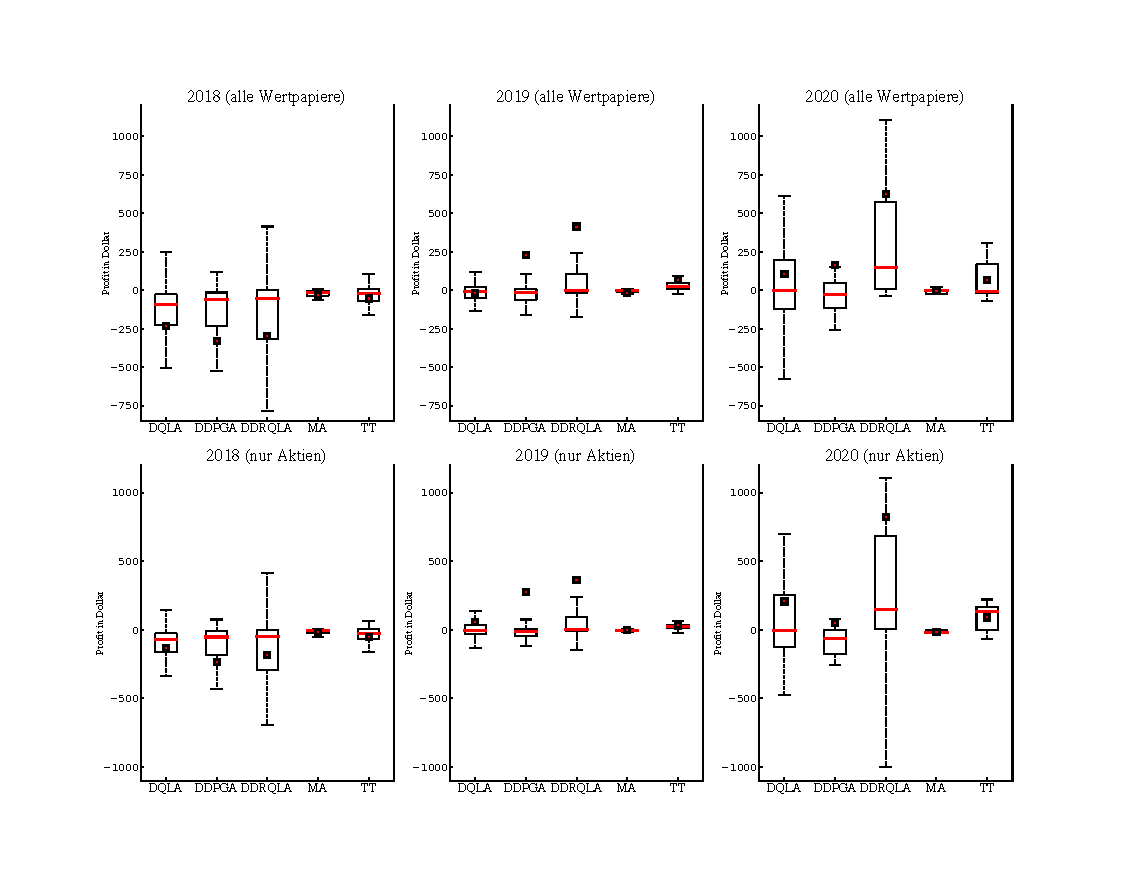
\includegraphics[scale=0.95]{figures/plot.pdf}
\vspace{0.1mm}
\caption[Ergebnisse der \acs{DRL} Agenten ohne Kontextdaten]{Ergebnisse aller 1440 Testdurchläufe der \acs{DRL} Agenten ohne Kontextdaten für alle Wertpapiere (oben) und nur für Aktien (unten) für jede Variante und jedes Evaluationsjahr. Die Kästen repräsentieren die Reichweite zwischen dem 25ten und 75ten Perzentil der Werte, während die Pfeile bis auf Ausreißer die gesamte Reichweite illustrieren. Der rote Punkt zeigt den Mittelwert und die rote Linie markiert den Median der Daten. Der Mittelwert weicht im zweiten Testjahr aufgrund hoher Ausreißer nach oben stark vom Median ab.}
  \label{fig:boxplot}
\end{figure}

Abbildung \ref{fig:boxplot} veranschaulicht die Verteilung der durchschnittlichen Ergebnisse jedes Agenten ohne Kontextdaten in Bezug auf deren Testjahr.
Agentenübergreifend ist zu sehen, dass durchschnittlich deutlich bessere Ergebnisse 2019 (145 \$) als 2018 (-185 \$) erreicht werden konnten.
Dieser Unterschied kann auf den längeren Trainingszeitraum und auf günstigere Marktbedingungen zurückgeführt werden.
Eine erste wichtige Erkenntnis daraus ist, dass durch eine gute Wahl des Testjahres die Agenten prozentual wesentlich weniger Verlust erleiden (42,0\%) als zuvor (65,3\%). Da selbst dieselben Agenten in unterschiedlichen Jahren hohe Varianzen in den Ergebnissen aufweisen, sind Performancevergleiche mit anderen Studien nur bei ähnlichem Setup sinnvoll.

Im Vergleich zu anderen Evaluationen mit kongruentem Testsetting schneiden die \acs{DRL} Varianten in den meisten Fällen leicht schlechter ab.
Für das Jahr 2018 liegt das beste Testergebnis auf einer Technologieaktie bei ungefähr 9\% Portfoliosteigerung, was weit unter den ca. 17\% von Théate et al. \parencite{théate2020application} liegt, die allerdings einen viel aufwendigeren Agenten und geringere Transaktionskosten verwenden.
Das beste Ergebnis im Jahr 2019 erzielte wie zu erwarten der \acs{DDRQLA} mit einem Gewinn von über 12\%, was auf der anderen Seite relativ nahe an die präsentierten Ergebnisse von \parencite{zhang2019deep,duel} herankommt.
Es gilt aber zu beachten, dass nicht state-of-the-art Ergebnisse erzielt werden sollen, sondern schwerpunktmäßig faire Vergleiche einzelner Varianten und Wertpapiercluster gemacht werden.

\paragraph{Vergleich der Agenten.}
Die großen Performanceunterschiede einzelner Varianten im oberen Teil von Abbildung \ref{fig:boxplot} zeigen, dass in der differenzierten Evaluation keine Architektur eindeutig bessere Ergebnisse liefert.
Während 2019 eine überlegene durchschnittliche Performance des \acs{DDRQLA} vor anderen \acs{DRL} Architekturen und den beiden Baseline Agenten beobachtet werden kann, schneidet er 2018 deutlich schlechter ab.
Trotz der hohen Varianz der Testergebnisse ist allerdings der Mittelwert des Sharpe Ratios der rekurrenten Variante in beiden Jahren am besten.
Dahinter weisen \acs{DDPG} Modelle durchschnittlich die besten Resultate auf, obwohl 2018 der \acs{DQLA} leicht dominiert. Dessen bessere Ergebnisse sind auf eine geringere Standardabweichung des Portfoliowertes zurückzuführen. Dies weist auf eine niedrigere Handelsfrequenz hin, was insbesondere geringere Verluste in moderaten Abschwungphasen wie in 2018 impliziert.

\paragraph{Vergleich der Charakteristika.}
Eine unerwartete Beobachtung dieser Studie ist, dass mit Aktien höhere Gewinne erzielt werden als mit Warentermingeschäften oder ETFs (siehe den unteren Teil von Abbildung \ref{fig:boxplot}).
In einer näheren Betrachtung werden Charakteristika in der Zeitreihe untersucht, mit denen die besseren Ergebnisse begründet werden können. 
Es zeigt sich, dass sowohl das Sharpe Ratio als auch die Performance signifikant\footnote{Konkret wird getestet, ob der gemittelte Profit für jede Komposition aus Agent und Wertpapier signifikant mit der Volatilität zusammenhängt.
Der Korrelationskoeffizient beträgt ca. -0,33.}
negativ mit der Volatilität einer Anlage korrelieren.
Dadurch dass Aktien mit 0,68 die geringste Standardabweichung gegenüber Waren (4,85) und ETFs (0,72) aufweisen, sind diese Anlagen in diesem Evaluationssetting vorteilhaft.
Genauer profitieren der \acs{DQLA} und der \acs{DDPGA} am meisten von der geringeren Volatilität, wohingegen der \acs{DDRQLA} 2019 sogar schlechter abschneidet.
Die Fähigkeit, besser auf alte Informationen durch die \acs{LSTM} Architektur zuzugreifen, scheint ausschlaggebend für eine gute Performance bei instabilen Wertentwicklungen zu sein.
Indes unterliegen stabile Wertpapiere weniger Spekulationen und Irregularitäten, womit die insgesamt bessere Mustererkennung erklären könnte.
Nicht signifikant ins Gewicht fällt hingegen der Kursverlauf eines Wertpapiers. 
Erwartungsgemäß beeinflusst ein wachsender Kursverlauf die Performance leicht positiv, ist aber zumindest in diesem Kontext nicht hinreichend für bessere Ergebnisse und zeigt ferner keinen signifikanten Zusammenhang mit der Performance.

Diese Schlussfolgerungen gelten für alle Charakteristika bis auf den Vergleich einzelner Branchen. 
In diesem Fall schneiden die Agenten 2019 bei Aktien von Unternehmen aus dem Gesundheitswesen trotz einer geringeren Volatilität und einer höheren Wertsteigerung schlechter ab.
Um diesen Zusammenhang zu untersuchen, wird der Einfluss des Beta-Faktors auf die Portfolioentwicklung für den Branchenvergleich zusätzlich untersucht.
Da Aktien aus dem Gesundheits- oder Finanzwesen einen niedrigen Beta-Faktor besitzen, korrelieren sie weniger stark mit dem Markt als Technologieaktien.
Diese Eigenschaft ist bei Aufwärtstrends wie beispielsweise im Jahr 2019 vorteilhaft, wenngleich Verluste in Abwärtstrends dadurch verstärkt werden.
Allgemein lässt sich in den Ergebnissen eine statistisch signifikante Abhängigkeit zwischen der Varianz des Portfolios und dem Beta-Faktor messen.
Demnach sollten Wertpapiere mit einem hohen Beta-Faktor nur bei einer risikofreudigen Nutzenfunktion eingesetzt werden. Für ein maximales Sharpe Ratio sollten jedoch Aktien gemieden werden, die sowohl eine hohe Volatilität als auch einen hohen Beta-Faktor besitzen. 

\section{Anwendung während der COVID-19 Pandemie}
\label{sec:covid}

Die rechten Schaubilder in Abbildung \ref{fig:boxplot} zeigen die überraschend gute Performance in Krisenzeiten.
Jede \acs{DRL} Variante erzielt in fast allen Fällen bessere Ergebnisse als die Baseline Agenten und weist sogar einen deutlich erhöhten Profit im Vergleich zum ersten Evaluationsjahr auf.
Nur die \acs{DDPG} Agenten weisen leicht schlechtere Tendenzen bei Aktien auf, speziell der \acs{DDPGAK} reduziert seine Handelsfrequenz auffällig drastisch. Eine mögliche Erklärung dafür ist der stark erhöhte \acs{^VIX}, der in den Trainingsjahren häufig positiv mit Verlusten korreliert.

\begin{figure}[t!]
\center
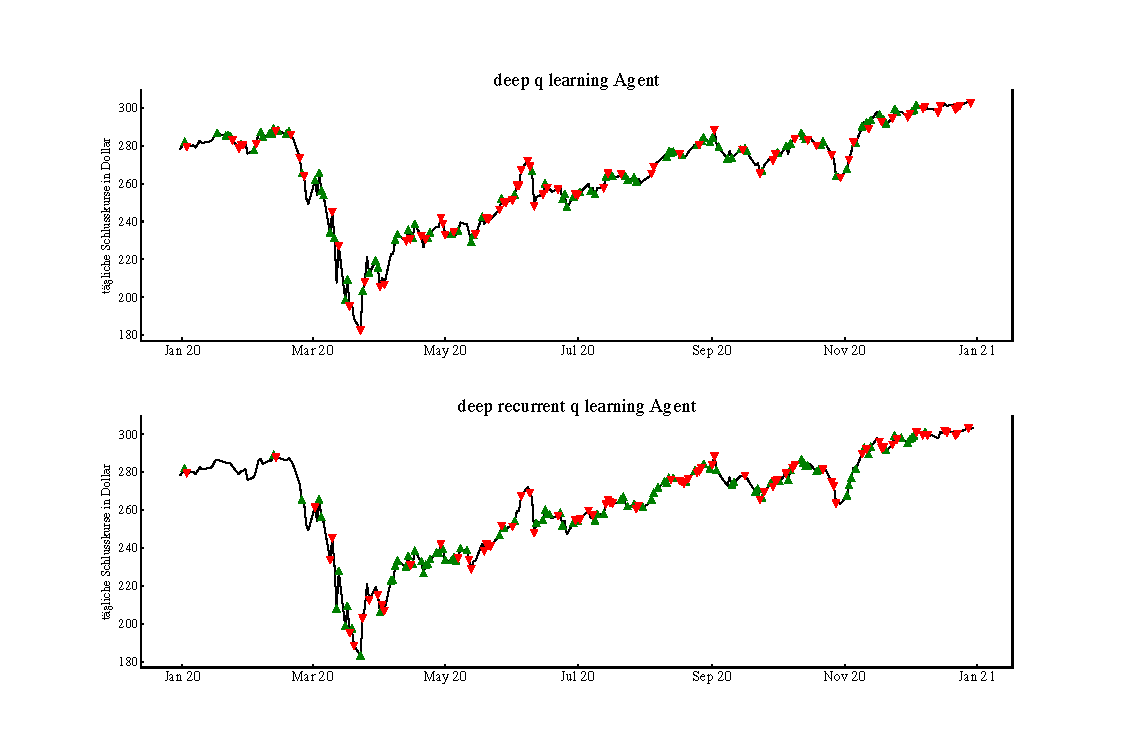
\includegraphics[scale=0.95]{figures/plot2.pdf}
\vspace{0.1mm}
\caption[Handlungsentscheidungen zweier Agenten während der COVID-19 Krise]{Ergebnisse des \acs{DQLA} (oben) und des \acs{DDRQLA} (unten). Die roten Pfeile signalisieren Verkaufszeitpunkte, grüne Pfeile zeigen Kaufzeitpunkte.}
  \label{fig:agentenspectime}
\end{figure}

Die beiden Schaubilder in Abbildung \ref{fig:agentenspectime} zeigen, wie sich die Handlungsentscheidungen des \acs{DDRQLA} und \acs{DQLA} der volatilen Krisenphase voneinander im Einzelnen unterscheiden:
Die Handlungen beider Agenten bleiben verzögert hinter dem Markttrend zurück. Jedoch reagiert der \acs{DDRQLA} besonders im ersten Quartal relativ früh auf die volatile Marktsituation, indem er seine Handelsfrequenz reduziert. Somit können hohe Verluste im späteren Verlauf vermieden werden.
Die deutlich bessere Rendite des \acs{DDRQLA} kann dadurch erklärt werden, dass anschließend im zweiten Quartal die günstige Marktsituation durch ein erhöhtes Kaufverhalten besser genutzt wird. 
Während der \acs{DQLA} sein tendenziell konservatives Kaufverhalten beibehält, profitiert der \acs{DDRQLA} von einer gierigen Strategie.
Diese Erkenntnis deckt sich mit den Schlussfolderung aus Abschnitt \ref{sec:erghaupteval}, dass die in Paragraph \ref{subsec:ddrqltheorie} beschriebenen Vorteile von \acs{LSTM} Schichten in volatilen Phasen deutlich die Performance verbessern.
Ferner kann der rekurrente Agent die Unterstützungszone\footnote{Eine Unterstützungszone ist ein Begriff in der technischen Analyse von Finanzdaten. Er beschreibt ein Niveau, bei dem ein sinkender Wertpapierkurs dazu tendiert, nach oben abzuprallen. Wird dieses Niveau durchbrochen, ist es wahrscheinlich, dass der Wertpapierkurs weiter fällt.} im vierten Quartal besser erkennen, aber aufgrund der Einschränkung des Aktionsraums nicht schnell genug seinen Bestand erhöhen.

Trotz einer erhöhten Volatilität sind die Agenten bei großen Marktveränderungen profitabel. 
Allerdings kann man wegen des eher kleinen Krisen-Datensatzes nicht gesichert von einer guten Performance in jeder Krisenzeit ausgehen. 
Da die Kurseinbrüche im ersten Quartal des Jahres eintreten, halten die Agenten aufgrund der strengen Handelsrestriktionen häufig nicht genügend Wertpapiere.
Für eine genauere Einschätzung muss in weiteren Studien der Testzeitraum der COVID-19 Pandemie variieren, damit die Auswirkungen des Kurseinbruchs in diversen Szenarien untersucht werden können.

\section{Einfluss der erweiterten Aspekte}
\label{sec:erweiterteragent}

Um detailliertere Erkenntnisse zu gewinnen, beschränkt sich die folgende Analyse auf Vergleiche zwischen Agenten, die denselben Trainingsalgorithmus verwenden.

\paragraph{Kontextdaten.}
Das Hinzufügen von Kontextdaten verbessert weder die Performance des \acs{DDPG} Algorithmus (\acs{DDPGAK}) noch des erweiterten \acs{DQL} Ansatzes (\acs{EDQLA}) in signifikantem Maße.
Obwohl für den \acs{DDPGAK} eine leicht bessere Performance in 2018 beobachtet wird, schneidet der Agent 2019 und 2020 schlechter ab.
Im Vergleich dazu erleidet der \acs{EDQLA} in den meisten Fällen durchschnittlich höhere Verluste, wobei allgemein ein instabileres Training mit einer signifikant längeren Laufzeit beobachtet werden kann.
Eine erhöhte Varianz sowohl bei der Validation als auch bei den Testergebnissen zeigt, dass die ergänzenden Marktinformationen in diesen simplen Modellen nicht vorteilhaft für die Entscheidungsfindung sind. 
Nichtsdestoweniger suggeriert eine qualitative Analyse der Handelszeitpunkte eine insgesamt geringfügig bessere Entscheidungsfindung in volatilen Phasen, die sich in einer reduzierten Handelsfrequenz bemerkbar macht.
Daraus lässt sich ableiten, dass Kontextdaten bei risikoreichen Konjunkturphasen unterstützend wirken können.
Da aber auch bei positivem Marktwachstum eine signifikant geringere Handelsfrequenz zu beobachten ist, können günstige Marktsituationen nur bedingt genutzt werden.

Wenngleich aufwendigere Agenten in einem anderen Setting \parencites{paperrepo2,startrader} mit Kontextdaten bessere Ergebnisse erzielen, 
können in dieser Evaluation durch korrelierende Marktinformationen keine signifikanten Unterschiede in der Performance beobachtet werden.
Gegeben, dass die zusätzlichen Finanzmarktdaten in großem Maße die Anzahl der Eingabewerte erhöhen, lohnt sich diese Modifikation aufgrund der höheren Komplexität unter den Limitationen von Kapitel \ref{ch:evaluationsaufbau} somit nicht.

\paragraph{Dropout.}

Änderungen in der Dropoutrate ändern nicht signifikant die Performance der modifizierten \acs{DQL} Variante, jedoch konnte das beste Ergebnis des Agenten in allen drei Jahren durch einen höheren Dropoutwert verbessert werden.
Da die Mittelwerte der Validations- und Testergebnisse weniger stark voneinander abweichen, lässt sich ein tendenziell weniger überangepasstes Modell beobachten.
Limitiert sind diese Schlussfolgerungen allerdings dadurch, dass der Effekt von Dropout nicht isoliert betrachtet werden kann.
Um genauere Aussagen über die Überanpassung des Modells zu treffen, müsste in einem gesonderten Experiment der \acs{DQLA} nur um die Regularisierungsmethode erweitert und den Einfluss auf die Performance statistisch analysiert werden. 
Das stellt ein interessantes zukünftiges Forschungsfeld dar, ist aber im Umfang dieser Bachelorarbeit nicht enthalten.

\paragraph{Aktionsraum.}

Die Erweiterung des Aktionsraums wirkt sich nicht signifikant auf die Performance des \acs{EDQLA} aus, aber führt besonders im Krisenjahr aufgrund eines deutlich erhöhten Wertpapierbestandes im ersten Quartal 2020 zu schlechteren Resultaten. 
Trotz schwächerer Handelseinschränkungen kann der \acs{DQL} Algorithmus ähnlich wie in Abbildung \ref{fig:agentenspectime} den Aufwärtstrend im zweiten Quartal nicht nutzen.
Stattdessen sorgt das erweiterte Framework dafür, dass wegen höherer Transaktionskosten volatile Phasen noch stärker die Performance beeinträchtigen.
Statistisch kann ein erhöhter Korrelationskoeffizient um $41\%$ für den negativen Zusammenhang der Volatilität mit der Performance nachgewiesen werden.

Allgemein investiert der Agent deutlich mehr, wodurch wie zu erwarten auch stärkere Ausreißer nach unten zu beobachten sind.
Der Agent kann demnach die in Abschnitt \ref{sec:erweiterung} beschriebene Handelseinschränkung überwinden und einen größeren Teil seines Bargeldes nutzen, besitzt aber dadurch höhere Varianzen in den Ergebnissen. 
Folglich besitzt der Agent ein durchschnittlich geringeres Sharpe Ratio als der einfachere \acs{DQLA}.
Eine wichtige Folgerung aus diesem Experiment ist daher, dass bei einem simplen \acs{DQL} Algorithmus mehr Handelsmöglichkeiten zu höherem Risiko führen.
Allerdings mindern Transaktionskosten hohe Gewinne, weshalb diese Erweiterung für das verwendete Modell nicht eingesetzt werden sollte.





\chapter{Fazit}
\label{ch:fazit}

In dieser Arbeit wurden eine wirklichkeitsnahe Evaluationsumgebung entwickelt, um in einer groß angelegten Studie empirisch verschiedene \acs{DRL} Architekturen und Implementierungen für den algorithmischen Handel differenziert zu analysieren.
Das vorgestellte Testsetting stellt Standards in der Hyperparametersuche und dem Design der Agenten auf, 
sodass damit ausführlich Effekte einzelner Wertpapiercharakteristika und Designänderungen bei unterschiedlichen Marktverhältnissen evaluiert werden konnten.

Die Auswertung der Hyperparametereinflüsse ergab keine eindeutige Struktur.
Jedoch lässt sich aus der Konfiguration der Modelle folgern, dass eine automatische Hyperparametereinstellung für jede Komposition aus Agent, Wertpapier und Zeithorizont ein wichtiger Bestandteil des Trainings darstellt.
Eine zentrale Erkenntnis dabei ist, dass die Verwendung einer größeren Schichtgröße signifikant positiv mit der Handelsfrequenz korreliert, was zu besseren Ergebnissen in moderaten Aufschwungphasen führte.
Überraschend erwies sich der Einsatz des Parameters $\tau$ für den \acs{DDPG} Algorithmus als unwichtig in diesem Setting.

Aus den Testergebnissen lässt sich ableiten, dass die tatsächliche Performance der Agenten stark von der Wahl des Wertpapiers und des Testjahres abhängt.
Insgesamt konnten sich verschiedene Varianten des \acs{DQL} Algorithmus gegenüber anderen \acs{DRL} Ansätzen und zwei Baseline Agenten durchsetzen.
Keine \acs{DQL} Variante zeigt allerdings eine signifikant bessere Performance gegenüber dem standardmäßigen \acs{DQL} Ansatz. Jedoch weisen in volatilen Phasen Netzwerke mit einer \acs{LSTM} Schicht eine bessere Entscheidungsfindung auf, während in Rezessionen naivere Ansätze besser abschneiden.
Speziell die Kombination aus einer Dueling Strategie und einer \acs{LSTM} Schicht erzielte sowohl ein besseres Sharpe Ratio als auch einen höheren durchschnittlichen Profit. 

Allgemein stellt sich die Volatilität eines Wertpapiers als entscheidendste Charakteristik heraus, gefolgt vom Beta-Faktor.
Während eine hohe Volatilität abträglich für eine gute Performance ist, erhöht ein größerer Beta-Faktor signifikant die Varianz des Portfolios.
Bessere Ergebnisse anderer Wertpapiercluster konnten auf die Wechselwirkung dieser beiden Eigenschaften zurückgeführt werden.
Modifikationen im Design wie die Eingabe zusätzlicher Marktinformationen, ein erweiterter Aktionsraum oder die Implementierung von Dropout erweitern das Modell, ohne in diesem Setting für den \acs{DDPG} oder \acs{DQL} Algorithmus signifikant die Performance zu verbessern.
Im Speziellen reduzieren die korrelierenden Eingabewerte die Handelsfrequenz signifikant, was bei volatilen Marktgeschehnissen unterstützend, hingegen bei Aufschwungphasen hinderlich ist.
Weiterhin wurde gezeigt, dass schwächere Handelsbeschränkungen durch einen größeren Aktionsraum insbesondere aufgrund hoher Transaktionskosten für die simplen Modelle zu erhöhtem Risiko und durchschnittlich mehr Verlusten führten.

Der algorithmische Handel unterliegt einer hohen Irregularität im Vergleich zu anderen Anwendungsfeldern von \acs{NN}en. 
Dies stellt eine Hürde für Investoren dar, da die tatsächliche Performance der Modelle stark von gewählten Zeiträumen, Wertpapieren und Konfigurationen abhängt.
Mit dieser Studie wurde versucht, einige Vermutungen bzgl. Hyperparametern, Wertpapierclustern und Modifikationen empirisch für simple \acs{DRL} Varianten zu untersuchen.
In weiteren Studien könnten komplexere \acs{DRL} Architekturen analysiert werden, um noch detaillierter die Wechselwirkungen von Wertpapiercharakteristika und den sequentiellen Entscheidungsprozess des algorithmischen Handels zu erkunden.
Beispielsweise könnte der Effekt von Kontextdaten auf ein aufwendigeres Modell mit einem komplexeren \acs{NN} isoliert erforscht werden.
Insbesondere könnten möglicherweise andere \acs{DRL} Varianten oder tiefere Netzwerke besser in der Lage sein, die multidimensionalen Muster der korrelierenden Marktinformationen zu erkennen. Es steht noch aus, Effekte von weiteren Kontextdaten wie z.B. Sentimentdaten oder fiskalpolitischen Maßnahmen experimentell zu überprüfen.
Dank der entwickelten Testumgebung lassen sich diese Modifikationen vielseitig evaluieren, sodass weitere Intuitionen mit umfassenden experimentellen Ergebnissen wissenschaftlich gestützt werden können.

Während die realitätsnahe Testumgebung eine differenziertere Evaluation als zuvor beschriebene Studien ermöglicht, kann sowohl der Datensatz als auch die Konfiguration der Modelle noch umfassender verfeinert und erweitert werden.
Erstens gibt es eine endlose Anzahl an Charakteristika, die man zusätzlich in die Testumgebung inkludieren könnte. Abgesehen von den untersuchten Wertpapierclustern könnten noch weitere Zusammenhänge mit Eigenschaften wie der Eigenkapitalquote, der Dividendenrendite oder des Streubesitzes zu signifikanten Unterschieden in der Performance führen.
Zweitens würde ein erschöpfenderes Hyperparametertuning (vgl. \parencites{snoek2012practical,bergstra2012random}) für bessere Ergebnisse und genauere Schlussfolgerungen sorgen. Damit wäre es insbesondere möglich, beispielsweise das fANOVA Framework \parencite{pmlr-v32-hutter14} zu verwenden, um detailliertere Einsicht in die Bedeutung von Hyperparametern und deren Interaktionen zu erhalten.
Drittens verwendet das einheitliche Framework bereits einige Implementationen, die den Lernprozess stabiler machen und gleichzeitig die Gefahr von Überanpassung reduzieren. Anpassungen in der Risikoadjustierung, etwa durch eine andere Belohnungsfunktion, könnten untersucht werden, um die starken Oszillationen im Training und die Schwankungen in den Ergebnissen zu reduzieren. Weight decay \parencite{ying2019overview} oder spezifischere Regularisierungsverfahren \parencites{zaremba2015recurrent} sind neben Dropout ebenfalls Methoden, mit denen bessere out-of-sample Ergebnisse erzielt werden könnten.
In weiteren Studien könnte es deshalb von Interesse sein, durch diese Implementierungen homogenere Ergebnisse zu erhalten und für eine bessere Konvergenz im Training zu sorgen. Das benötigt allerdings eine aufwendige, individuelle Anpassung jedes Modells und ist daher nicht im Rahmen dieser Bachelorarbeit enthalten.














\chapter*{Anhang}
\addcontentsline{toc}{chapter}{Anhang}
\label{ch:anhang}
\vspace{-5mm}
\section*{Tabelle A1: Liste der Agenten}
\label{tabe1}

Zu sehen ist eine vollständige Liste aller fünfzehn verwendeter \acs{DRL} Varianten und der zwei Baselines. Die ersten vier Varianten werden näher untersucht.
Die Agenten sind entsprechend ihrer Performance in der Vorstudie sortiert. Deep curiosity q learning und verschiedene Modifikationen davon verwenden einen weiteren \acs{DRL} Algorithmus, der unter anderem in \parencite{10.5555/1671238} näher erläutert wird. Aufgrund der schlechteren Performance in der Vorstudie im Vergleich zu anderen Implementierungen wird auf diese Varianten daher nicht näher eingegangen. Außerdem erweist sich die Double Strategie (cf. \parencite{vanhas}) als nicht Vorteil für den algorithmischen Handel in diesem Setting.
\vspace{1mm}
\begin{table}[h!]
\label{fig:table1h}
\begin{adjustwidth}{-.8in}{0in}
  \begin{center}
  \hline
  \vspace{5}
	\begin{tabular}{l}
	duel deep recurrent q learning\\
	deep q learning\\
	deep deterministic policy gradient\\
	deep deterministic policy gradient mit Kontextdaten\\
	\vspace{-2mm}\\
	deep recurrent q learning\\
	double duel deep recurrent q learning\\
	deep recurrent deterministic policy gradient\\
	double deep recurrent q learning\\
	duel deep q learning\\
	duel deep recurrent deterministic policy gradient\\
	double duel deep q learning\\
	deep recurrent curiosity q learning\\
	duel deep curiosity q learning\\
	double deep q learning\\
	duel deep deterministic policy gradient\\
	deep curiosity q learning\\
	turtle trading\\
	moving average
	  \vspace{8}
    \end{tabular}
    \hline
    \vspace{10}
  \end{center}
  \end{adjustwidth}
\end{table}
\vspace{-3mm}
\section*{Tabelle A2: Datensatz}
\label{tabe2}
\addcontentsline{lot}{table}{A1~~~Vollständige Liste aller \acs{DRL} Varianten}

Der nachstehende Datensatz umfasst alle Wertpapiere für die Vorstudie (grau hinterlegt), die Hauptevaluation und des Krisenjahres (unterstrichen). Weiterhin sind Kontextdaten enthalten, die dem \acs{DDPGAK} und dem \acs{EDQLA} zusätzlich übergeben werden.
Die Wertpapiere werden zur besseren Übersicht in Wertpapierklassen und Börsen unterteilt. Absätze gruppieren die Wertpapiere hinsichtlich des Sektors, der Unternehmensgröße und der Region. Hinter den geschweiften Klammern steht der weitere Vertreter des Sektors, dessen Wertentwicklung beim Handel mit Wertpapieren dieses Sektors zusätzlich in den Kontextdaten enthalten sind.
\enlargethispage{2\baselineskip}
\vspace*{-4mm}%
\begin{table}[!b]
\label{tab:allassets}
\begin{adjustwidth}{-.8in}{-.5in}
\rule{19.4cm}{1}\vspace{-3mm}
\begin{minipage}[t]{.48\linewidth}
\centering
\footnotesize
\label{tab:first_table}
\begin{tabular}{ll}
\header{~~~Ticker}  &  \header{Unternehmen} \\   
\midrule

\textbf{Aktien (USA)}
\vspace*{1.6mm}\\
~~~\colorbox{grey!20}{ORCL}	&\colorbox{grey!20}{Oracle}\hspace{8em}\rdelim\}{16.4}{17.5mm}[\parbox{12.5mm}{\scriptsize{Broadcom\\(AVGO)}}]\\
~~~\colorbox{grey!20}{AAPL} 	&\colorbox{grey!20}{Apple}\\
~~~~ACN	& Accenture\\
~~~~MSFT	& Microsoft\\
~~~~IBM	& IBM\\
~~~~CSCO	& Cisco~~~~~~~~~~~~~~~~~~~~~~~~~~~~~~~~~~~~~~~~~~~~~~~\\
~~~~NVDA	& Nvidia\\
~~~~ADBE	& Adobe\\
~~~~HPQ	& HP\\
~~~~\underline{INTC}	& \underline{Intel}  
\vspace*{1.4mm}\\
~~~~TESS	& TESSCO Technologies\\
~~~~ASYS	& Amtech Systems\\
~~~~CTG	& Computer Task Group\\
~~~~BELFB	& Bel Fuse\\
~~~~AVNW	& Aviat Networks\\
~~~~LYTS	& LSI Industries
\vspace*{1.4mm}\\
~~~\colorbox{grey!20}{\underline{JPM}}	& \colorbox{grey!20}{\underline{JPMorgan Chase}}\hspace{1em}\rdelim\}{3}{17.5mm}[\parbox{12.5mm}{\scriptsize{Blackrock\\(BLK)}}]\\
~~~~BAC	& Bank of America\\
~~~\colorbox{grey!20}{\underline{V}} & \underline{Visa Inc.}
\vspace*{1.4mm}\\
~~~\colorbox{grey!20}{PFE}	& 	\colorbox{grey!20}{Pfizer}\hspace{7em}\rdelim\}{3}{17.5mm}[\parbox{12.5mm}{\scriptsize{AstraZeneca\\(AZN)}}]\\
~~~~MRK	& 	Merck \& Co.\\
~~~~JNJ		& Johnson \& Johnson
\vspace*{1.4mm}\\
~~~\colorbox{grey!20}{CAJ}	& 	\colorbox{grey!20}{Canon}\hspace{7.5em}\rdelim\}{9.5}{17.5mm}[\parbox{120mm}{\scriptsize{China Telecom\\(CHA)}}]\\
~~~~\underline{NICE}	& 	\underline{NICE}\\
~~~~TSM	& 	Taiwan Semiconductor\\
~~~~SNE	& 	Sony\\
~~~~UMC	& 	United Microelectronics\\
~~~~CHKP	& 	Check Point Software
\vspace*{1.4mm}\\
~~~~SILC	& 	Silicom\\
~~~~GILT	& 	Gilat Satellite Networks\\
~~~~TSEM	& 	Tower Semiconductor
\vspace*{1.4mm}\\
~~~~LFC	& 	China Life Insurance\hspace{1em}\rdelim\}{3}{17.5mm}[\parbox{120mm}{\scriptsize{Nomura Holdings\\(NMR)}}]\\
~~~~\underline{SMFG}	& 	\underline{Sumitomo Mitsui} \\
~~~~SHG	& 	Shinhan
\vspace*{1.4mm}\\
~~~~NOK	& 	Nokia\hspace{5em}\rdelim\}{6}{17.5mm}[\parbox{120mm}{\scriptsize{STMicroelectronics\\(STM)}}]\\
~~~~ASML	& 	ASML\\
~~~~ERIC	& 	LM Ericsson\\
~~~~SAP	& 	SAP\\
~~~~TEL	& 	TE Connectivity\\
~~~~LOGI	& 	Logitech
\vspace*{1.4mm}\\
~~~\colorbox{grey!20}{HSBC}	& 	\colorbox{grey!20}{HSBC}\hspace{5em}\rdelim\}{3}{17.5mm}[\parbox{120mm}{\scriptsize{Credit Suisse\\(CS)}}]\\
~~~~ING	& 	ING\\
~~~~BCS	& 	Barclays\\

\end{tabular}
\end{minipage}%
\begin{minipage}[t]{.5\linewidth}
\centering
\footnotesize
\label{tab:first_table}
\begin{tabular}{ll}
\header{~~~Ticker}  &  \header{Unternehmen} \\ 

\midrule

\textbf{Aktien (Asien)}
\vspace*{1.6mm}\\
~~~~0992.HK	& 	Lenovo Group\hspace{1em}\rdelim\}{3}{17.5mm}[\parbox{120mm}{\scriptsize{Tencent\\(0700.HK)}}]\\
~~~~3888.HK	& 	Kingsoft\\
~~~~0763.HK	& 	ZTE
\vspace*{1.4mm}\\
~~~~0939.HK	& 	China Construction Bank\hspace{0.4em}\rdelim\}{3}{17.5mm}[\parbox{120mm}{\scriptsize{China Merchants Bank\\(3968.HK)}}]\\
~~~~2318.HK	& 	Ping An Insurance\\
~~~~0998.HK	& 	China CITIC Bank
\vspace*{3.3mm}\\

\textbf{ETF's}
\vspace*{1.6mm}\\
~~~~\underline{DIA}	& 	\underline{Dow Jones}\hspace{1.7em}\rdelim\}{3}{17.5mm}[\parbox{120mm}{\scriptsize{NYSE Composite\\( $\hat{}$ NYA)}}]\\
~~~~SPY	& 	S\&P 500\\
~~~~QQQ		& 	NASDAQ
\vspace*{1.4mm}\\
~~~\colorbox{grey!20}{EWJ}	& 	\colorbox{grey!20}{Nikkei 225}\hspace{7em}\rdelim\}{3}{17mm}[\parbox{120mm}{\scriptsize{HANG SENG Index\\( $\hat{}$ HSI)}}]\\
~~~~EWT		& 	iShares MSCI Taiwan\\
~~~~\underline{EWY}	& 		\underline{iShares MSCI South Korea}
\vspace*{1.4mm}\\
~~~~\underline{EZU}	& 	\underline{FTSE 100}\hspace{4.5em}\rdelim\}{3}{17.5mm}[\parbox{120mm}{\scriptsize{IBEX\\(IBEX)}}]\\
~~~~CAC.PA	& 	Lyxor CAC 40\\
~~~~EXS1.DE	& 	iShares Core DAX
\vspace*{1.4mm}\\
~~~~EXXY.MI	& iShares Diversified Commodity\hspace{0.3em}\rdelim\}{2}{17.5mm}[\parbox{120mm}{\scriptsize{iShares S\&P GSCI\\(GSG)}}]\\
~~~~DBC		& 	Invesco DB Commodity Index~~~~~~~~~~~~~~~~~~~~~~~~~~
\vspace*{3.3mm}\\

\textbf{Waren}
\vspace*{1.6mm}\\
~~~\colorbox{grey!20}{GC=F} 	& 	\colorbox{grey!20}{Gold}\hspace{3em}\rdelim\}{4}{17.5mm}[\parbox{120mm}{\scriptsize{Aluminum\\(ALI=F)}}]\\
~~~~SI=F	& 	Silver\\
~~~~PL=F	& 	Platinum\\
~~~~HG=F	& 	Copper
\vspace*{1.4mm}\\
~~~\colorbox{grey!20}{\underline{CL=F}}	& 	\colorbox{grey!20}{\underline{Crude Oil}}\hspace{3em}\rdelim\}{4}{17.5mm}[\parbox{120mm}{\scriptsize{Brent Crude Oil\\(BZ=F)}}]\\
~~~~HO=F	& 	Heating Oil\\
~~~~NG=F	& 	Natural Gas\\
~~~~RB=F	& 	RBOB Gasoline
\vspace*{1.4mm}\\
~~~~HE=F	& 	Lean Hogs\hspace{3em}\rdelim\}{3}{17.5mm}[\parbox{120mm}{\scriptsize{Class III Milk\\(DC=F)}}]\\
~~~~LE=F	& 	Live Cattle\\
~~~~GF=F	& 	Feeder Cattle\\
~~~~\underline{DC=F}	& 	\underline{Class III Milk} $\longrightarrow$ ~\scriptsize{Live Cattle (LE=F)} 
\vspace*{1.4mm}\\
~~~~ZC=F	& 	Corn\hspace{6em}\rdelim\}{4}{17.5mm}[\parbox{120mm}{\scriptsize{Cocoa\\(CC=F)}}]\\
~~~~ZS=F	& 	Soybean\\
~~~~KC=F	& 	Coffee\\
~~~~KE=F	& 	KC HRW Wheat
\vspace*{3.3mm}\\

\textbf{Kontextdaten}
\vspace*{2mm}\\
~~~~$\hat{}$ SPY & S\&P 500 Trust\\
~~~~$\hat{}$ TNX & Treasury Yield\\
~~~~$\hat{}$ VIX & Volatility Index\\
~~~~GC=F & Gold Feb 21

\end{tabular}
\end{minipage}%
\vspace*{1mm}
\\
\rule{19.4cm}{1}
\end{adjustwidth}
\vspace*{3mm}\\
\begin{adjustwidth}{-.2in}{-15in}
\captionsetup{width=1.15\textwidth}
\end{adjustwidth}
\end{table}
\addcontentsline{lot}{table}{A2~~~Übersicht über alle verwendeten Wertpapiere}

\microtypesetup{protrusion=false}
\microtypesetup{protrusion=true}
\printbibliography{}

\end{document}

